\documentclass[a4paper, 12pt]{report}

%%%%%%%%%%%%
% Packages %
%%%%%%%%%%%%
\usepackage{rest-api}
\usepackage[english]{babel}
\usepackage[noheader]{packages/sleek}
\usepackage{packages/sleek-title}
\usepackage{packages/sleek-theorems}
\usepackage{packages/sleek-listings}
\usepackage[most]{tcolorbox}


\usepackage{color}
\usepackage{tabularx}

\usepackage{pdfpages}

\definecolor{pblue}{rgb}{0.13,0.13,1}
\definecolor{pgreen}{rgb}{0,0.5,0}
\definecolor{pred}{rgb}{0.9,0,0}
\definecolor{pgrey}{rgb}{0.46,0.45,0.48}
\definecolor{tsyellow}{RGB}{255,185,88}

\usepackage{listings}
\lstset{language=Java,
 columns=fullflexible,
  showspaces=false,
  showtabs=false,
  frame=single,
  breaklines=true,
  postbreak=\mbox{\textcolor{red}{$\hookrightarrow$}\space},
  showstringspaces=false,
  breakatwhitespace=true,
  commentstyle=\color{pgreen},
  keywordstyle=\color{pblue},
  stringstyle=\color{pred},
  basicstyle=\ttfamily
}

\usepackage{enumitem,amssymb}

\newlist{todolist}{itemize}{2}
\setlist[todolist]{label=$\square$}

\newenvironment{boxexercise}
{\begin{tcolorbox}
[enhanced jigsaw,breakable,pad at break*=1mm,
 colback=tsyellow!20,boxrule=0pt,frame hidden]}
{\end{tcolorbox}}

\newenvironment{summary}
{\hspace{10pt}\par\small\it
 \begin{list}{}{\leftmargin=35pt\rightmargin=25pt}
 \item\ignorespaces\advance\baselineskip -1pt}
{\end{list}\vspace{-0.5cm}}

\newenvironment{remark}
{\vspace{0.5cm}\noindent\small\it
 \marginpar{\vspace{-3mm}
\includegraphics[width=1.0cm]{idea}}}
{\vspace{0.5cm}}

\newtheorem{envoefening}{\textbf{Oefening}}[chapter]
\newenvironment{oefening}
               {\begin{boxexercise}\begin{envoefening}}
               {\end{envoefening}\end{boxexercise}}
               
\newcommand*{\xml}[1]{\texttt{<#1>}}

%%%%%%%%%%%%%%
% Title-page %
%%%%%%%%%%%%%%

\logo{./resources/pdf/logo.png}
\institute{Hogeschool PXL}
\faculty{PXL-Digital}
%\department{Department of Anything but Psychology}
\title{Java Advanced\\An Introduction to Spring Boot}
\author{\textit{Author}\\Nele \textsc{Custers}}
%\supervisor{Linus \textsc{Torvalds}}
%\context{Well, I was bored...}
\date{\today}

%%%%%%%%%%%%%%%%
% Bibliography %
%%%%%%%%%%%%%%%%

\usepackage{biblatex}
\addbibresource{./resources/bib/references.bib}

%%%%%%%%%%
% Others %
%%%%%%%%%%

\lstdefinestyle{latex}{
    language=TeX,
    style=default,
    %%%%%
    commentstyle=\ForestGreen,
    keywordstyle=\TrueBlue,
    stringstyle=\VeronicaPurple,
    emphstyle=\TrueBlue,
    %%%%%
    emph={LaTeX, usepackage, textit, textbf, textsc}
}

\FrameTBStyle{latex}

\def\tbs{\textbackslash}

%%%%%%%%%%%%
% Document %
%%%%%%%%%%%%

\begin{document}
    \maketitle
    \romantableofcontents
    
 
  
\chapter{Introduction}
    
\fcolorbox{black}[HTML]{E9F0E9}{\parbox{\textwidth}{%
\noindent \textbf{Learning goals}\\
The junior-colleague
\begin{enumerate}[nolistsep]
\item can describe what Spring is
\item can describe what Spring Boot is
\item can explain what a three-tier application is
\item can identify the three layers in a Spring Boot application
\item can explain the responsibilities of the layers in a Spring Boot application
\item can explain the architecture of a Spring RESTful web application
\item can explain what a DTO is
\item can explain what an entity-object is
\item can explain what dependency injection is
\item can explain what a Spring bean is
\item can explain what a Spring container is
\item can explain what a Spring Boot starter is
\end{enumerate}}}


\section{Enterprise Applications with Java}

Spring Boot is een framework om enterprise applications te bouwen met Java.
Enterprise applicaties zijn applicaties die bedrijven bouwen of laten bouwen voor hun klanten en medewerkers.  Enterprise applicaties worden ontwikkeld om de bedrijfsprocessen te ondersteunen. 

Enterprise applicaties hebben specifieke kenmerken. Deze kenmerken komen voort uit de complexe aard en specifieke eisen van grootschalige bedrijfssystemen.  Enkele belangrijke kenmerken van enterprise applicaties vanuit het oogpunt van een ontwikkelaar:

\begin{itemize}
\item{Schaalbaarheid (scalability):} Enterprise applicaties moeten een groot aantal gebruikers en gegevens aankunnen.  Ontwikkelaars moeten de architectuur van de applicatie zodanig ontwerpen dat schalen mogelijk is om een groeiend aantal gebruikers en datavolumes aan te kunnen.

\item{Betrouwbaarheid en hoge beschikbaarheid:} Van enterprise applicaties wordt verwacht dat ze 24/7 beschikbaar zijn en snelle responstijden hebben.  Ontwikkelaars moeten oplossingen voorzien om problemen en downtime te voorkomen.  Ze moeten de betrouwbare werking van de applicatie kunnen garanderen.

\item{Beveiliging:} Enterprise applicaties verwerken gevoelige bedrijfsgegevens, waaronder financiële informatie, klantgegevens,...   Ontwikkelaars moeten robuuste beveiligingsmaatregelen implementeren,  zoals authenticatie,  autorisatie,  versleuteling van gegevens en audittrails,  om de gegevens te beschermen tegen ongeautoriseerde toegang.

\item{Integratie:} Enterprise applicaties moeten vaak worden geïntegreerd met verschillende bestaande systemen zoals databanken en externe services.  Voorbeelden van externe services zijn bijvoorbeeld betaalsystemen en boekhoudpakketten. Ontwikkelaars moeten zorgen voor een veilige en betrouwbare gegevensuitwisseling tussen verschillende enterprise applicaties. 

\item{Aanpasbaarheid en flexibiliteit:} Enterprise applicaties worden gebruikt door gebruikers uit diverse afdelingen en teams binnen een organisatie, elk met hun eigen unieke workflows en eisen. Ontwikkelaars moeten applicaties bouwen die kunnen worden aangepast en geconfigureerd om aan deze specifieke behoeften te voldoen. 
Enterprise applicaties ondergaan vaak veranderingen en updates op basis van veranderende zakelijke behoeften. Daarnaast veranderen de workflows en eisen van de gebruikers ook. 
Ontwikkelaars moeten verandering effectief beheren door versiebeheer, wijzigingstracering en terugrolmechanismen te implementeren.
Afhankelijk van de sector moeten enterprise applicaties voldoen aan specifieke wettelijke normen die doorheen de tijd kunnen veranderen. 

\item{Lange levenscyclus:} Enterprise applicaties hebben meestal een langere levenscyclus dan andere soorten software.  Ontwikkelaars moeten zorgen voor voortdurend onderhoud,  updates en verbeteringen.

\item{Samenwerking en documentatie:} Aangezien meerdere ontwikkelaars en teams mogelijk werken aan verschillende delen van een enterprise applicatie, zijn duidelijke code-documentatie, versiebeheer en samenwerkingsgerichte ontwikkelingspraktijken essentieel.

\item{Testen en kwaliteitsborging:} Grondig testen is essentieel voor enterprise applicaties om bugs, prestatieproblemen en beveiligingskwetsbaarheden te identificeren en aan te pakken. Ontwikkelaars moeten geautomatiseerd testen, unit testing, integratietesting en gebruikersacceptatietests implementeren.

\item{Gebruikerservaring (UX):} Hoewel functionaliteit cruciaal is, is een positieve gebruikerservaring ook belangrijk voor gebruikersacceptatie en productiviteit. Ontwikkelaars moeten streven naar intuïtieve interfaces en workflows die de tevredenheid van gebruikers vergroten.
\end{itemize}

Over het algemeen vereist de ontwikkeling van enterprise applicaties een uitgebreid begrip van bedrijfsprocessen, technische expertise en het vermogen om functionaliteit, prestaties, beveiliging en gebruikerservaring in evenwicht te brengen om te voldoen aan de unieke behoeften van grote organisaties.

In 1999 besliste Sun Microsystems om de programmeertaal Java uit te bereiden om het ontwikkelen van enterprise applicaties te vergemakkelijken.  Met de lancering van J2EE (Java 2 Enterprise Editie) en de applicatie servers om de J2EE-toepassingen op te deployen onstond een schaalbaar en betrouwbaar platform. 
J2EE,  dat wordt hernoemd naar Java EE (Java Platform, Enterprise Edition), verwijst naar een verzameling specificaties. Het bestaat uit een reeks standaarden en API's die ontwikkelaars gebruiken om de enterprise-software te implementeren. 

Wanneer in de tekst wordt verwezen naar "J2EE-specificaties" of "Java EE-specificaties", dan verwijst dit naar de reeks specificaties die Java EE vormen.  Deze specificaties zijn de  beschrijvingen van hoe bepaalde componenten en functionaliteiten in een enterprise Java-applicatie moeten worden geïmplementeerd.  Sun Microsystems en later Oracle, dat in de 2010 Sun Microsystems overneemt, zorgen steeds voor een bruikbare implementatie van hun specificaties. 

In een enterprise applicatie moet het mogelijk zijn om eenvoudig mails te versturen. Daarom werd dus de JavaMail API Design Specificaties uitgeschreven. Dit kan je zien als een uitgebreide analyse van de vereisten.  De Reference implementation is voorzien door Oracle

Yes, besides the JavaMail reference implementation, there are other implementations of the JavaMail API. While the reference implementation is provided by Oracle as part of the Java EE platform, alternative implementations have been developed by various organizations and communities. Some of these implementations include:

Apache Geronimo JavaMail: Apache Geronimo is an open-source application server project that includes its own implementation of the JavaMail API.

IBM WebSphere Application Server JavaMail: IBM's WebSphere Application Server also provides its own implementation of the JavaMail API.

JBoss AS (WildFly) JavaMail: The JBoss Application Server (now known as WildFly) includes its own implementation of the JavaMail API.

Google App Engine JavaMail: Google App Engine provides its own implementation of the JavaMail API tailored for its cloud platform.

Caucho Resin JavaMail: The Resin application server offers its own implementation of the JavaMail API.

These alternative implementations often aim to provide the same functionality as the JavaMail reference implementation while potentially offering additional features or optimizations.  


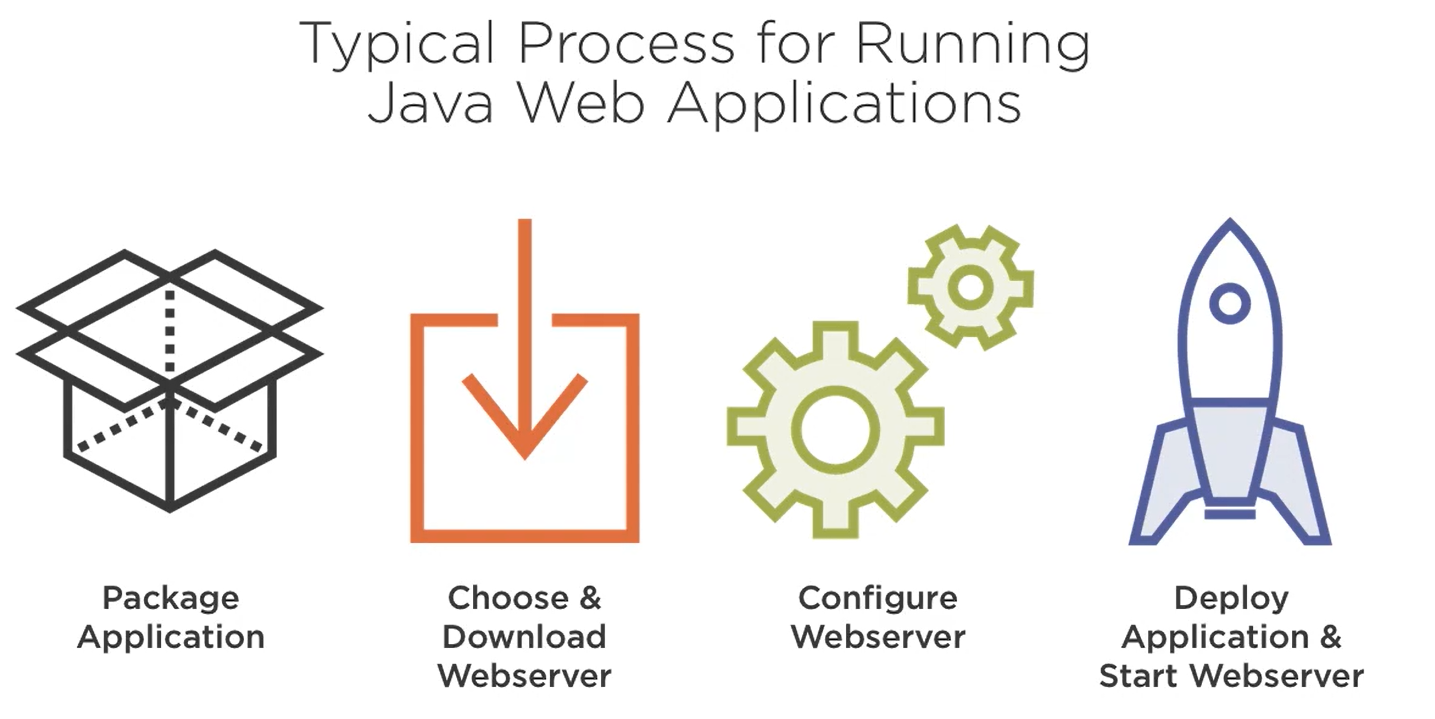
\includegraphics[width=\textwidth]{./images/chapter1/before_spring_boot.png} 

Spring came into being in 2003 as a response to the complexity of the early J2EE specifications. While some consider Java EE and its modern-day successor Jakarta EE to be in competition with Spring, they are in fact complementary. The Spring programming model does not embrace the Jakarta EE platform specification; rather, it integrates with carefully selected individual specifications from the traditional EE umbrella. Spring started as a lightweight alternative to Java Enterprise Edition. Rather than develop components as heavyweight Enterprise
JavaBeans (EJBs), Spring offered a simpler approach to enterprise Java development, utilizing dependency injection and aspect-oriented programming to achieve the capabilities of EJB with plain old Java objects (POJOs).
But while Spring was lightweight in terms of component code, it was heavyweight in terms of configuration. Initially, Spring was configured with XML (and lots of it).
It provides everything you need to create Java enterprise applications. Spring offers the flexibility to create many kinds of architectures depending on an application’s needs. As of Spring Framework 6.0, Spring requires Java 17+.

De lente ontstond in 2003 als reactie op de complexiteit van de vroege J2EE-specificaties. Hoewel sommigen Java EE en zijn moderne opvolger Jakarta EE als concurrenten van Spring beschouwen, zijn ze in feite complementair. Het Spring-programmeringsmodel omarmt niet de Jakarta EE platformspecificatie; in plaats daarvan integreert het met nauwkeurig geselecteerde individuele specificaties uit het traditionele EE-landschap. Spring begon als een lichtgewicht alternatief voor Java Enterprise Edition. In plaats van componenten te ontwikkelen als zware Enterprise JavaBeans (EJB's), bood Spring een eenvoudigere benadering voor enterprise Java-ontwikkeling, waarbij gebruik werd gemaakt van afhankelijkheidsinjectie en aspectgeoriënteerde programmering om de mogelijkheden van EJB te bereiken met gewone Java-objecten (POJO's).
Maar hoewel Spring lichtgewicht was qua componentcode, was het zwaar qua configuratie. In het begin werd Spring geconfigureerd met XML (en veel ervan).
Het biedt alles wat je nodig hebt om Java enterprise-applicaties te maken. Spring biedt de flexibiliteit om verschillende soorten architecturen te creëren, afhankelijk van de behoeften van een applicatie. Vanaf Spring Framework 6.0 vereist Spring Java 17+.

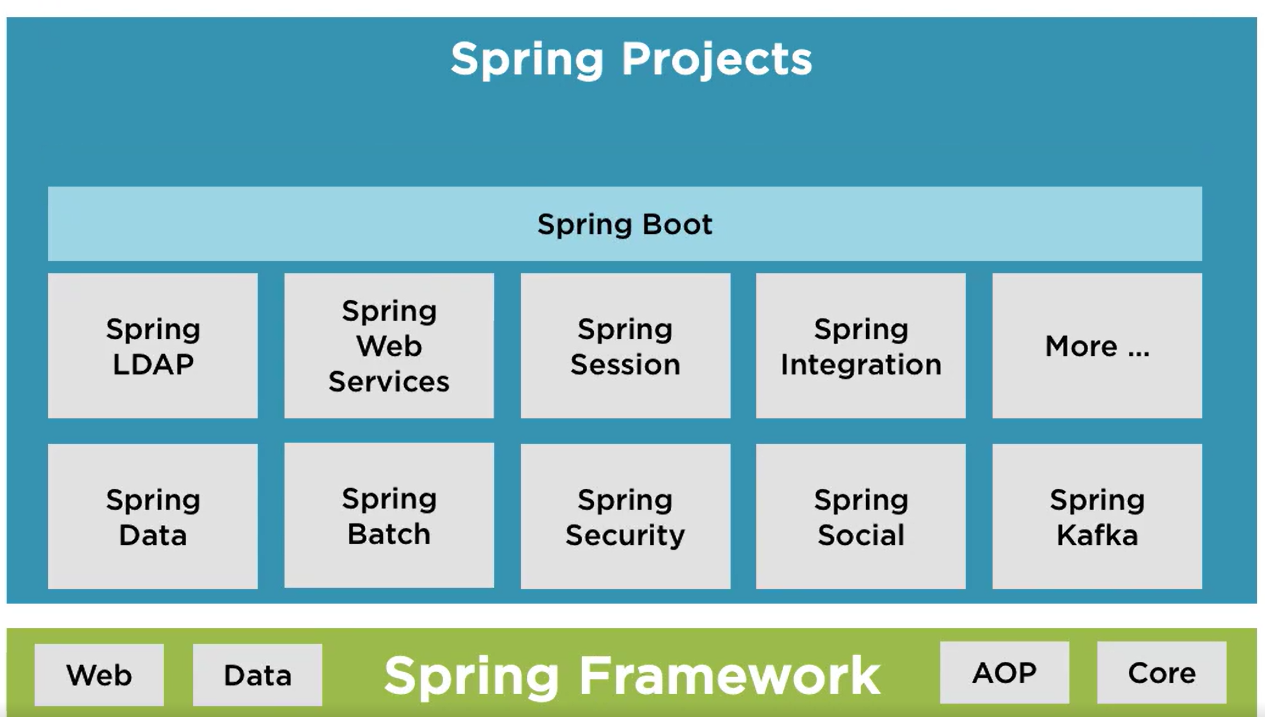
\includegraphics[width=\textwidth]{./images/chapter1/spring_framework.png} 

Spring Boot is a project that is built on the top of the Spring Framework. It provides an easier and faster way to set up, configure, and run java applications.

    
\section{What is Spring Boot?}
 
Spring Boot is an open-source Java framework to create production-ready,  standalone Spring applications. It's a robust, widely used framework. The creation of this framework was facilitated by the desire to simplify the development of applications on the popular Java EE technology stack from Oracle, which was very complex and difficult to use at the time. With very little configuration, you can create easily your first Spring Boot application.

Let's look at some advantages of Spring Boot for developers 
\begin{itemize}
\item speed up the process of creating and deploying application
\item create standalone applications with less or almost no configuration overhead
\item easy to learn framework
\item increase productivity of developers
\end{itemize}

\section{Bootstrapping a simple application}

\subsection{Using Spring Initializr}
Spring Initializr is a web application that can generate a Spring Boot project.
The url for this web application is \url{https://start.spring.io/}. You can select the necessary configuration, including the build tool, language, version of the Spring Boot framework, and any dependencies for your project. IntelliJ IDEA Ultimate provides the Spring Initializr project wizard that integrates with the Spring Initializr API to generate and import your project directly from the IDE.

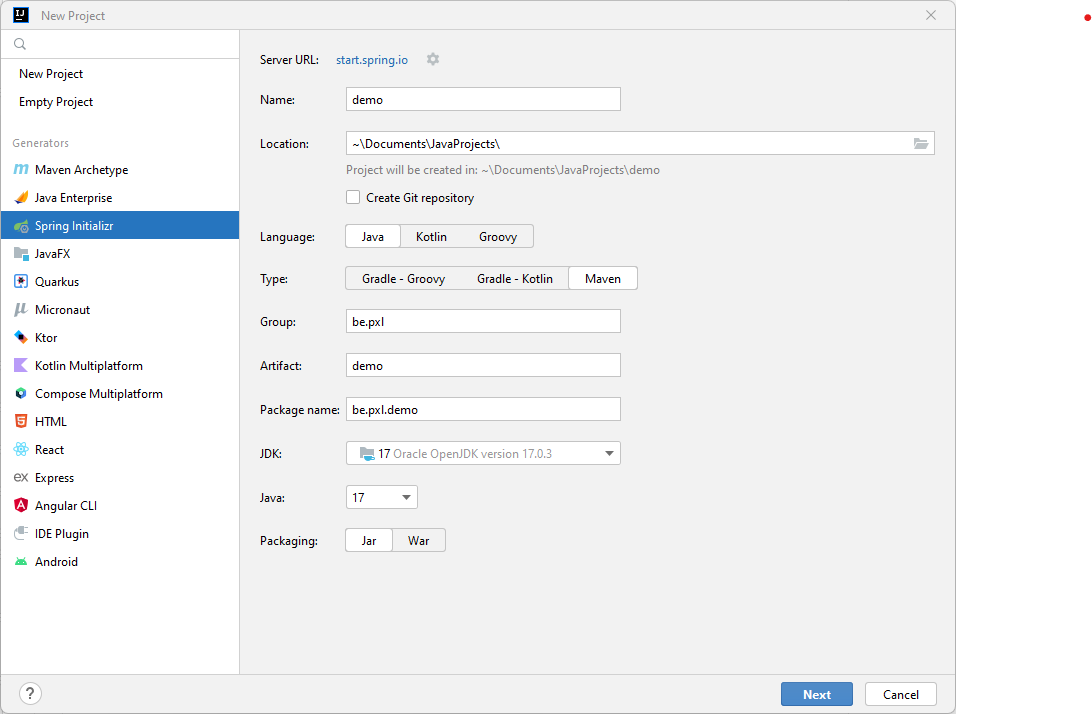
\includegraphics[width=\textwidth]{./images/chapter1/spring_initializer_intellij.png}

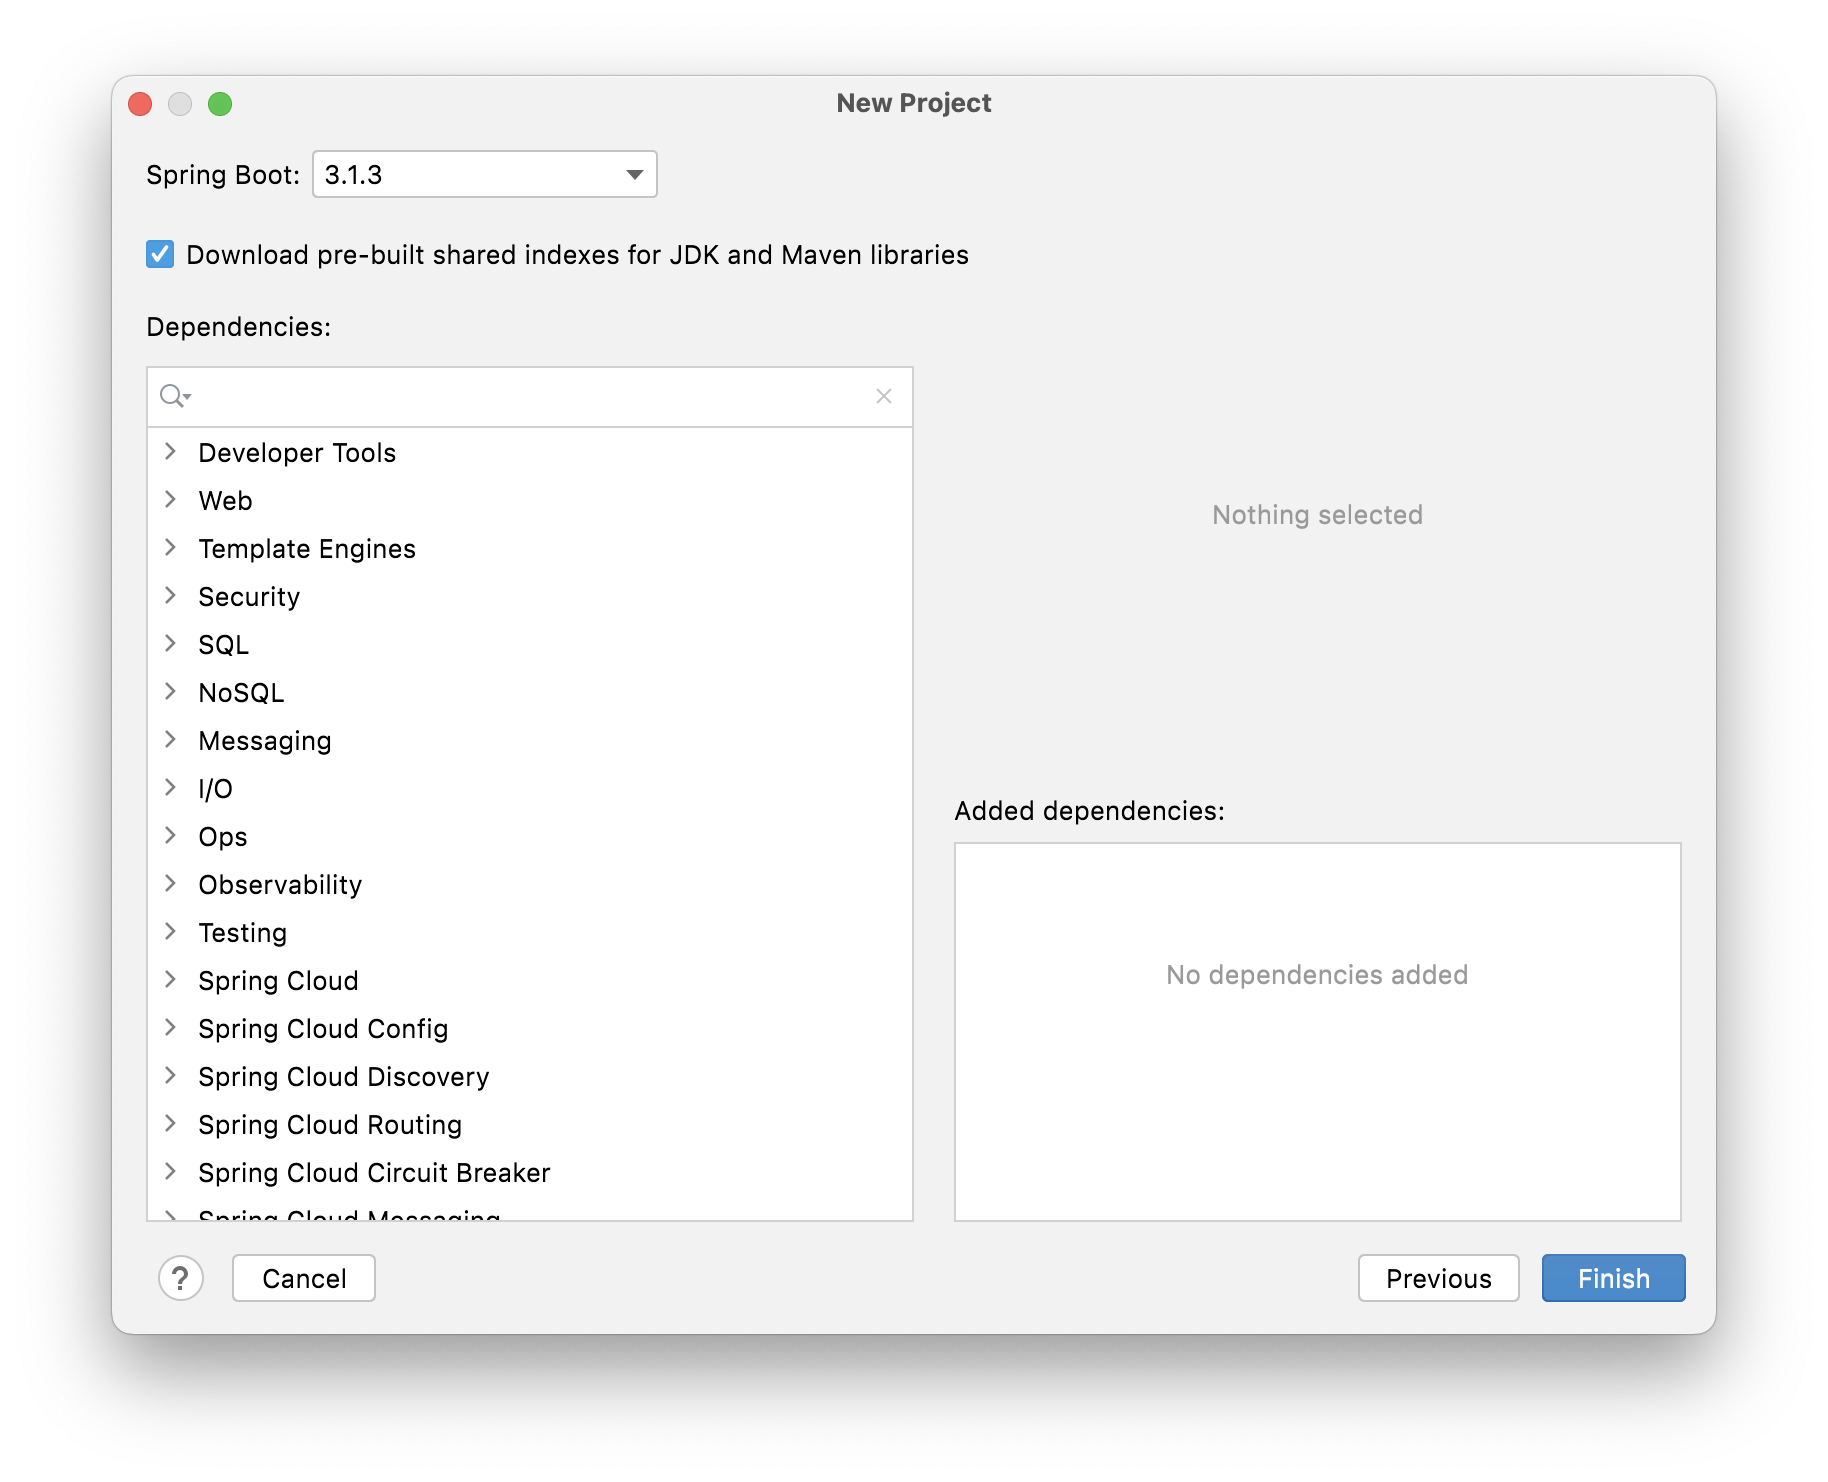
\includegraphics[width=\textwidth]{./images/chapter1/new_project.png}

We select Spring Web dependency. Spring Web uses Spring MVC. It is used for building RESTful Web Services. Spring MVC provides the annotation @RestController for classes that implement the REST endpoints.
To run a RESTful Web Service you need a web container. Spring Boot will automatically add an embedded Tomcat web container to your project. If you prefer another web container, you can update Spring Boot's configuration.
Finally Jackson is a popular third-party library for converting Java-objects to JSON and vice versa.

\begin{oefening}
Create the demo project. You can use the wizard in IntelliJ IDEA Ultimate or \url{https://start.spring.io/}.
\end{oefening}

\section{Running the demo project}

The starting point of a Spring Boot application is the class with the main-method and annotated with @SpringBootApplication.  This class can be found in the folder /src/main/java.  Spring Boot offers a lot of annotations to reduce the workload of developers.   

\begin{lstlisting}[frame=single]
package be.pxl.demo;

import org.springframework.boot.SpringApplication;
import org.springframework.boot.autoconfigure.SpringBootApplication;

@SpringBootApplication
public class DemoApplication {

    public static void main(String[] args) {
        SpringApplication.run(DemoApplication.class, args);
    }

}
\end{lstlisting}

By running the main-class you start your Spring Boot application. 

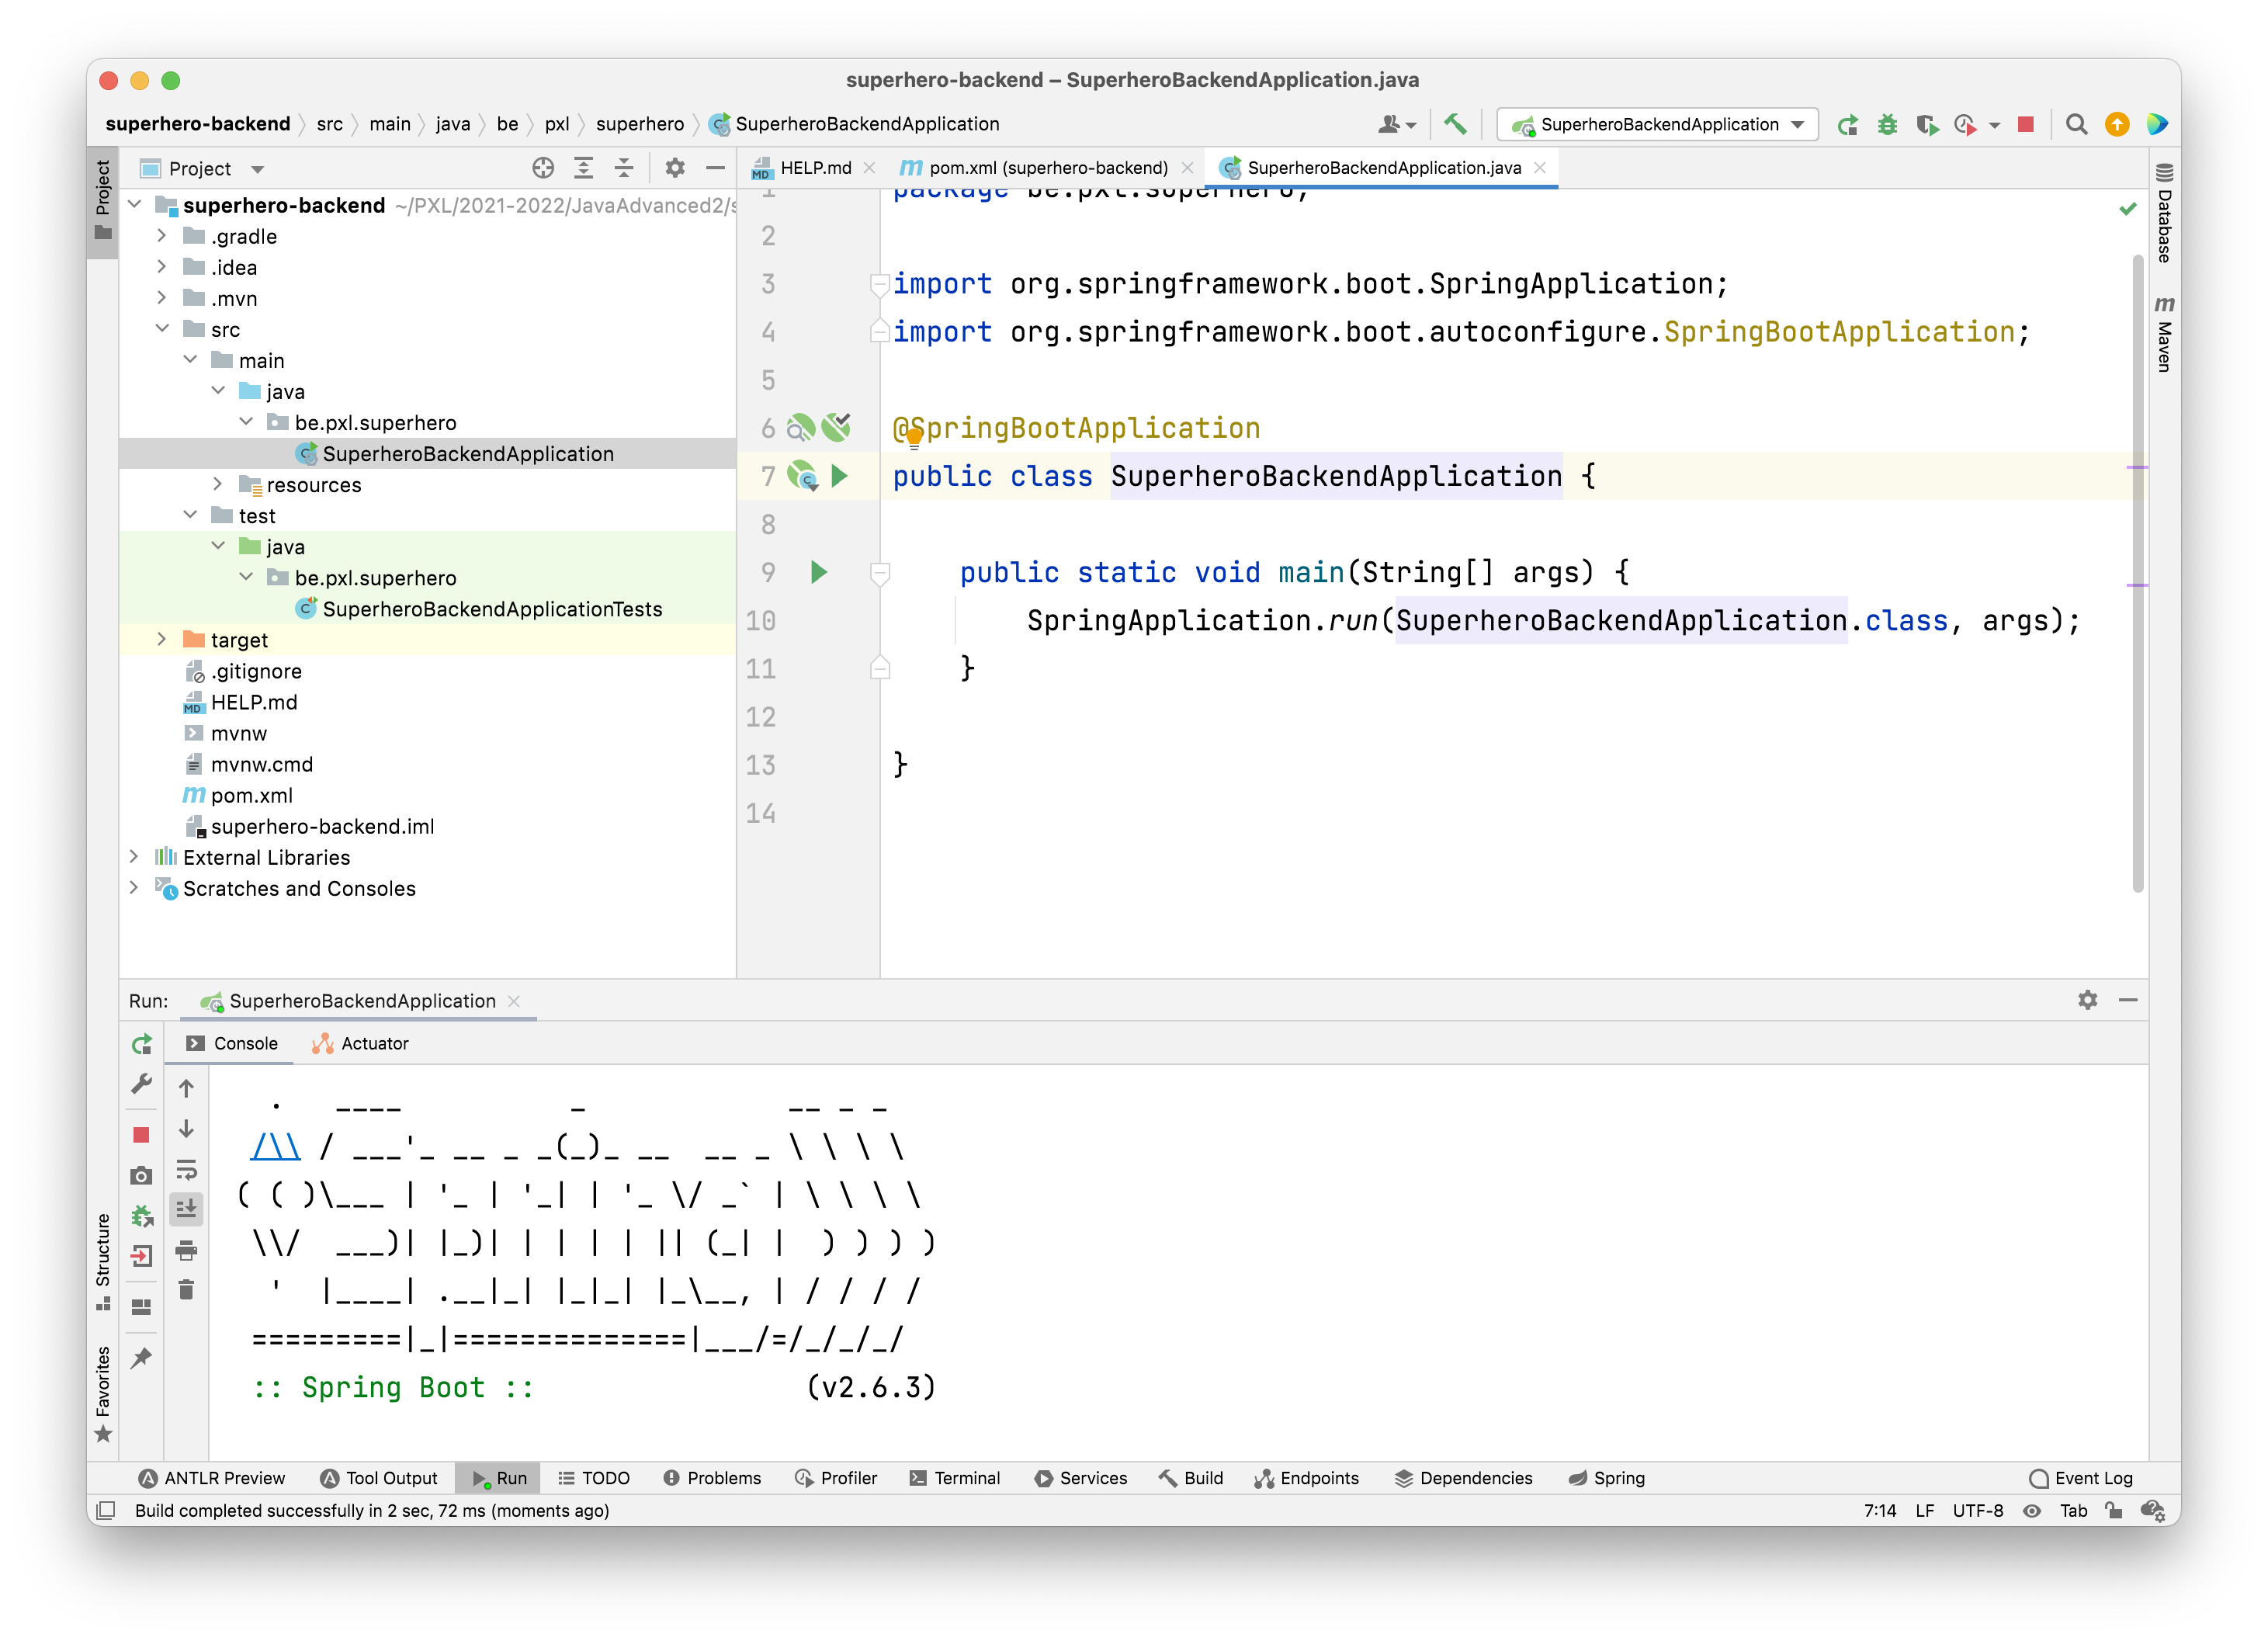
\includegraphics[width=\textwidth]{./images/chapter2/first-run.png}

Currently our Spring Boot application only shows a whitelabel error page. This error page is available when you perform a GET for URL \url{http://localhost:8080}.

\frame{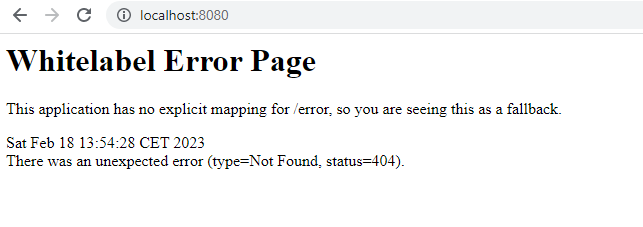
\includegraphics[width=\textwidth]{./images/chapter2/whitelabel_error_page.png}} 

Port 8080 is the default port. If this port is not available you will see an error message in Spring Boot's logging.

\begin{lstlisting}[frame=single]
***************************
APPLICATION FAILED TO START
***************************

Description:

Web server failed to start. Port 8080 was already in use.
\end{lstlisting}

The port number can be changed in the file application.properties. You have to add the property server.port here with the desired port number.

\begin{lstlisting}[frame=single]
server.port=8081
\end{lstlisting}

\subsection{Component}


\begin{lstlisting}
@Component
public class DependencyInjectionWithSpring implements CommandLineRunner {
   
   @Override    
   public void run(String... args) throws Exception {
	   System.out.println("Welcome to Java Advanced");
   }
}
\end{lstlisting}

De Spring Boot de CommandLineRunner interface voorziet de mogelijkheid om een stukje code uit te voeren zodra de Spring Boot applicatie ge\"initialiseerd is. 

Zodra je de CommandLineRunner interface implementeert in een klasse kan je de run-methode overschrijven. In de run-methode plaats je de code die uitgevoerd moet worden
als de applicatie opstart.  Zodra de Spring Boot applicatie opstart worden een aantal initialisatie-fasen doorlopen.  Eerst wordt de \textbf{application context} aangemaakt en alle Spring beans worden geladen. Als de applicatie volledige is ge\"initialiseerd wordt de run-methode van de CommandLineRunner automatisch door het Spring boot framework aangeroepen.



\subsubsection{Spring beans}

Spring Beans zijn componenten die volledig worden beheerd door het Spring Boot framework. Je hoeft zelf geen instanties van deze klassen te maken, Spring Boot genereert de objecten automatisch.  Daarnaast beheert Spring Boot ook de objecten. Wanneer een klasse gebruik wil maken van de functionaliteiten van een dergelijke Spring Bean, zal Spring Boot ervoor zorgen dat de instantie van de Spring Bean beschikbaar is voor de betreffende klasse.

\subsubsection{Application context}

De Application context is een belangrijk onderdeel van elke Spring Boot applicatie.
Hierin wordt namelijk bijgehouden welke infals een slimme doos waarin alle informatie en instellingen voor je Spring Boot-toepassing worden bewaard. Deze doos zorgt ervoor dat alle onderdelen van je applicatie met elkaar kunnen praten en weten waar ze moeten zoeken voor dingen zoals configuratie, gegevensbronnen en andere beans (componenten). Het maakt je Spring Boot-applicatie georganiseerd en helpt deze soepel te werken door alles op één plek te houden. Je kunt de application context beschouwen als het brein van je Spring Boot-applicatie dat alles coördineert en beschikbaar maakt voor de verschillende onderdelen van je programma.


Iets meer info tonen:

spring.application.name=My Demo

package be.pxl.demo.beans;

import org.springframework.boot.CommandLineRunner;
import org.springframework.context.ApplicationContext;
import org.springframework.stereotype.Component;

import java.time.LocalDateTime;
import java.time.ZoneId;
import java.time.ZoneOffset;

@Component
public class DependencyInjectionWithSpring implements CommandLineRunner {
	private final ApplicationContext applicationContext;

	public DependencyInjectionWithSpring(ApplicationContext applicationContext) {
		this.applicationContext = applicationContext;
	}

	@Override
   public void run(String... args) throws Exception {
	   System.out.println("Welcome to Java Advanced");
		System.out.println(applicationContext.getApplicationName());
		System.out.println(applicationContext.getDisplayName());
		System.out.println(applicationContext.getId());
		LocalDateTime dateTime = convertStartupDateToLocalDateTime(applicationContext.getStartupDate());
		System.out.println(dateTime);
		System.out.println(LocalDateTime.now());
   }


   private LocalDateTime convertStartupDateToLocalDateTime(long startupDate) {
	   // Get the system's default timezone
	   ZoneId systemZoneId = ZoneId.systemDefault();
	   // Get the ZoneOffset for the system's default timezone
	   ZoneOffset systemZoneOffset = systemZoneId.getRules().getOffset(LocalDateTime.now());
		return LocalDateTime.ofEpochSecond(applicationContext.getStartupDate() / 1000, 0, systemZoneOffset);

   }
}



Spring Boot Application Context:
When your Spring Boot application starts, it goes through various phases of initialization. After the application context is prepared and all beans are loaded, any classes implementing CommandLineRunner are executed.

\subsection{The Maven pom file}

POM stands for \'Project Object Model\'. It is an XML representation of a Maven project held in a file named pom.xml. This file can be found in your project directory. The POM contains all necessary information about a project, as well as configurations of plugins to be used during the build process. We will cover Maven in chapter 3.

\begin{lstlisting}[frame=single]
<?xml version="1.0" encoding="UTF-8"?>
<project xmlns="http://maven.apache.org/POM/4.0.0" xmlns:xsi="http://www.w3.org/2001/XMLSchema-instance"
         xsi:schemaLocation="http://maven.apache.org/POM/4.0.0 https://maven.apache.org/xsd/maven-4.0.0.xsd">
    <modelVersion>4.0.0</modelVersion>
    <parent>
        <groupId>org.springframework.boot</groupId>
        <artifactId>spring-boot-starter-parent</artifactId>
        <version>3.0.2</version>
        <relativePath/> <!-- lookup parent from repository -->
    </parent>
    <groupId>be.pxl</groupId>
    <artifactId>demo</artifactId>
    <version>0.0.1-SNAPSHOT</version>
    <name>demo</name>
    <description>demo</description>
    <properties>
        <java.version>17</java.version>
    </properties>
    <dependencies>
        <dependency>
            <groupId>org.springframework.boot</groupId>
            <artifactId>spring-boot-starter-web</artifactId>
        </dependency>

        <dependency>
            <groupId>org.springframework.boot</groupId>
            <artifactId>spring-boot-starter-test</artifactId>
            <scope>test</scope>
        </dependency>
    </dependencies>

    <build>
        <plugins>
            <plugin>
                <groupId>org.springframework.boot</groupId>
                <artifactId>spring-boot-maven-plugin</artifactId>
            </plugin>
        </plugins>
    </build>
</project>
\end{lstlisting}

spring-boot-starter-parent is a starter project that provides the default configuration for spring-based applications. Here you choose the version of Spring Boot.

For large projects, managing the dependencies is not always easy. Spring Boot solves this problem by grouping certain dependencies together. These groups of dependencies are called starters. All Spring Boot starters are named following the same naming pattern. The all start with spring-boot-starter-*, where * indicates the purpose and functionality provided by the starter.

spring-boot-starter-web adds all the libraries we need to develop web components. An embedded server will be provided in the Spring Boot project. Therefore the environment where the Spring Boot project is executed does not need to have a pre-installed server. The default embedded server for Spring Boot is Tomcat. The Spring MVC framework which provides all classes for developing RESTful web services is also part of spring-boot-starter-web.

spring-boot-starter-test (with scope test) is the starter for testing Spring Boot applications with libraries including JUnit Jupiter, Hamcrest and Mockito.

Inversion of Control (IoC) is \'e\'en van de basisprincipes van het Spring framework.
Bij Inversion of Control is het aanmaken en beheren van objecten niet langer de verantwoordelijkheid van de objecten zelf, maar is er een aparte 

So, Inversion of Control is about shifting the responsibility of managing object interactions from your code to a higher-level component (the framework or container). This makes your code more modular and flexible, as you rely on the framework to provide and coordinate the necessary components, 

To explain this in layman's terms, suppose you drive a car to your work place. This means you control the car. The IoC principle suggests to invert the control, meaning that instead of driving the car yourself, you hire a cab, where another person will drive the car.

What is a Bean in Spring Boot? A Bean is an object that is managed by the Spring framework. It is created, managed, and managed by the Spring container. Beans can be used to encapsulate and provide services, utilities, and functionalities to other components in an application.

In Spring, the objects that form the backbone of your application and that are managed by the Spring IoC container are called beans. A bean is an object that is instantiated, assembled, and otherwise managed by a Spring IoC container. Otherwise, a bean is simply one of many objects in your application.

TODO add image





IOC en dependency injection 


@Component
public class DependencyInjectionWithSpring implements CommandLineRunner {
   
   @Autowired
   private WeatherService weatherService;
   
   @Override    
   public void run(String... args) throws Exception {
	   weatherService.printWeather();
   }
}

WeatherService.java

import org.springframework.stereotype.Component;

@Component
public class WeatherService {
   public void printWeather() {
      System.out.println("The weather is sunny with a 20% chance of rain");
   }
}


Exercise

Create the class 





\subsection{@SpringBootApplication}

Java annotations are a mechanism for adding metadata information to our source code. An annotation processor processes these annotations at compile time or runtime to provide functionality such as code generation, error checking, etc.

@SpringBootApplication annotation is used to enable following three features:
\begin{itemize}
\item @EnableAutoConfiguration: enable Spring Boot’s auto-configuration mechanism
\item @ComponentScan: enable @Component scan on the package where the application is located
\item @Configuration: allow to register extra beans in the context or import additional configuration classes
\end{itemize}


\subsection{Auto-configuration}

Spring Boot auto-configuration attempts to automatically configure your Spring application based on the dependencies that you have added.
To gain some insight in this auto-configuration let's add a line in the application.properties file. This file can be found in the directory /src/main/resources. 

\begin{lstlisting}
logging.level.org.springframework=debug
\end{lstlisting}

logging.level.org.springframework is a application properties. A list of all available application properties can be found at \url{https://docs.spring.io/spring-boot/docs/current/reference/html/application-properties.html}.

\begin{oefening}
Add the line above to the application.properties file and restart the Spring Boot application.
\end{oefening}

In the console you will find all the auto-configuration Spring Boot is doing.

\chapter{REST}

\fcolorbox{black}[HTML]{E9F0E9}{\parbox{\textwidth}{%
\noindent \textbf{Learning goals}\\
De junior-collega
\begin{enumerate}[nolistsep]
\item kan beschrijven wat een RESTful web applicatie is
\item kan een POST, GET, PUT en DELETE-verzoek afhandelen in Spring Boot
\item kan beschrijven wat spring-boot-starter-web is
\item 
\end{enumerate}}}

\section{HTTP-verzoekmethoden}

Spring Boot is een goede keuze als je een REST API (of voluit een RESTful web API) wilt ontwikkelen in Java.

REST (Representational State Transfer) is een gestandaardiseerde manier om communicatie tussen verschillende softwaretoepassingen over het internet mogelijk te maken. 
In een RESTful web applicatie wordt de functionaliteit van de applicatie beschikbaar gesteld als resources, die kunnen worden geïdentificeerd door URI's (Uniform Resource Identifiers).  Gebruikers en andere applicaties kunnen met deze resources communiceren via standaard HTTP-verzoekmethoden (HTTP-request, HTTP-method of HTTP-verb). In essentie is HTTP het transportprotocol dat wordt gebruikt om gegevens over te dragen,  terwijl REST de verzameling van ontwerpprincipes is die bepalen hoe die gegevens moeten worden georganiseerd en benaderd.

\begin{itemize}
\item \textbf{GET}: Het GET-verzoek wordt gebruikt om gegevens op te halen van een specifieke resource. 

Voorbeeld URI: GET /api/products/123

Dit verzoek haalt informatie op over het product met ID 123.

\item \textbf{POST}: Het POST-verzoek wordt gebruikt om nieuwe gegevens naar een resource te verzenden. Het wordt vaak gebruikt voor het maken van nieuwe resources of het toevoegen van gegevens aan een bestaande resource.

Voorbeeld URI: POST /api/products

Dit verzoek voegt een nieuw product toe aan de lijst van producten.

\item \textbf{PUT}: Het PUT-verzoek wordt gebruikt om gegevens bij te werken voor een specifieke resource of om een nieuwe resource te maken als deze niet bestaat. Het is idempotent, wat betekent dat meerdere PUT-verzoeken hetzelfde resultaat opleveren.

Voorbeeld URI: PUT /api/products/123

Dit verzoek bijwerken de informatie van het product met ID 123.

\item \textbf{DELETE}: Het DELETE-verzoek wordt gebruikt om een resource te verwijderen of te deactiveren.

Voorbeeld URI: DELETE /api/products/123

Dit verzoek verwijdert het product met ID 123 uit de lijst van producten.
\end{itemize}

\section{Spring Boot Starter Web}

Spring Boot Starter Web is de verzameling van alle bibliotheken (third party libraries) die we nodig hebben om RESTful web applicaties te bouwen.  De verzameling bestaat ondermeer uit Spring MVC,  REST,  jackson en Tomcat. 
Apache Tomcat is een populaire open source web server voor Java toepassingen.  Als je de dependency spring-boot-start-web toevoegt, start de Tomcat web server op zodra je de Spring boot applicatie opstart.  We spreken van de "embedded web server" in Spring boot.  Je kan er ook voor kiezen om  \'e\'en van de alternatieve web servers te gebruiken zoals jetty of undertow. 
Jackson is een populaire library om Java-objecten naar JSON te converteren en vice versa.

\begin{lstlisting}
<dependency>
		<groupId>org.springframework.boot</groupId>
		<artifactId>spring-boot-starter-web</artifactId>
</dependency>
\end{lstlisting}
		
Je voegt de dependency toe in het bestand pom.xml.
		
Start nu de Spring Boot applicatie opnieuw op.

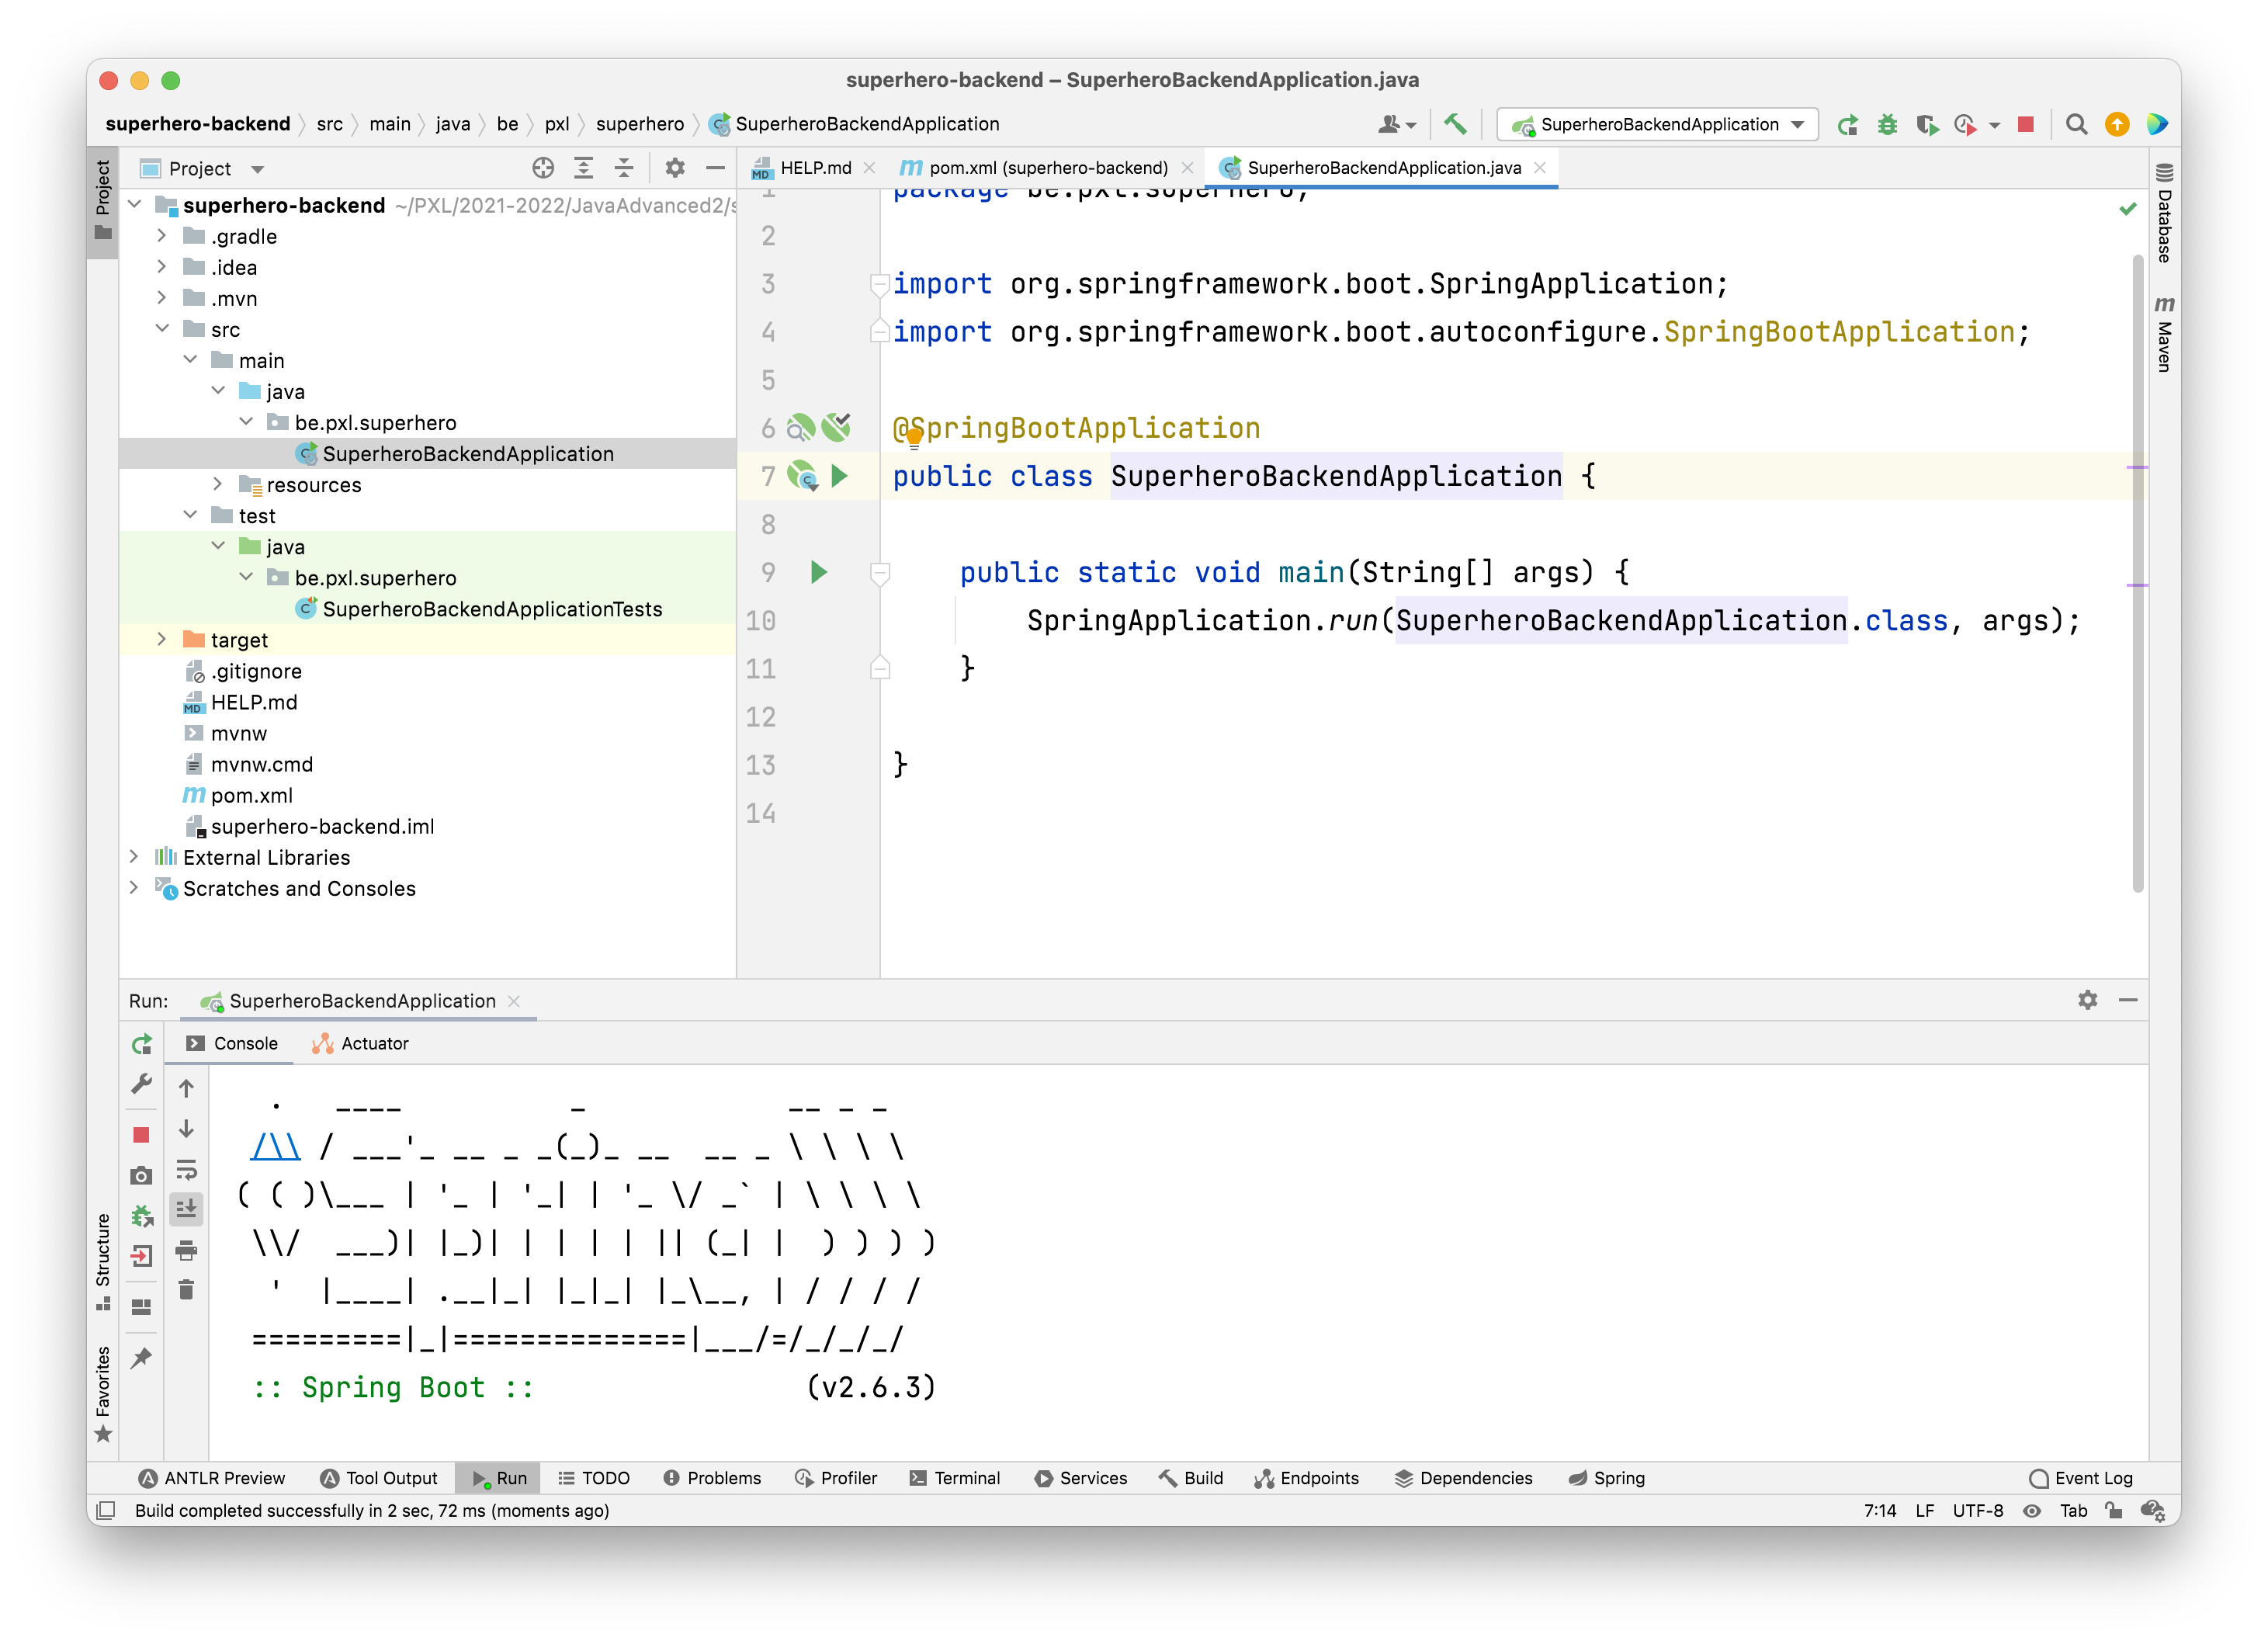
\includegraphics[width=\textwidth]{./images/chapter2/first-run.png}

Momenteel kan de Spring Boot applicatie enkel een whitelabel error pagina tonen.  De error pagina krijg je te zien als je een GET-request uitvoert voor URL \url{http://localhost:8080}.

\frame{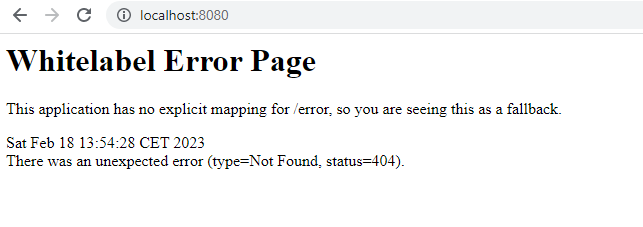
\includegraphics[width=\textwidth]{./images/chapter2/whitelabel_error_page.png}} 

Poort 8080 is de default poort van de Tomcat webserver.  Als deze poort al gebruikt wordt door een ander programma, krijg je de volgende foutmelding te zien.

\begin{lstlisting}[frame=single]
***************************
APPLICATION FAILED TO START
***************************

Description:

Web server failed to start. Port 8080 was already in use.
\end{lstlisting}

De poortnummer kan aangepast worden in het bestand application.properties.  Je gebruikt de eigenschap \textbf{server.port} om de gewenste poortnummer te kiezen.

\begin{lstlisting}[frame=single]
server.port=8081
\end{lstlisting}

\section{De RestController}

Spring boot heeft een annotatie voorzien voor de Spring bean die verantwoordelijk is voor het afhandelen van HTTP requests nl. @RestController. Spring boot heeft ook een annotatie @Controller, maar de @RestController zorgt ervoor dat het respons op het HTTP-request automatisch wordt omgezet (geserialiseerd) naar JSON of XML en wordt teruggestuurd naar de client.


\begin{lstlisting}[frame=single]
package be.pxl.demo.api;

import jakarta.annotation.PostConstruct;
import org.springframework.web.bind.annotation.GetMapping;
import org.springframework.web.bind.annotation.RestController;

import java.util.ArrayList;
import java.util.List;
import java.util.Random;

@RestController
@RequestMapping("/greetings")
public class GreetingController {

    private final List<String> messages = new ArrayList<>();
    private static final Random RANDOM = new Random();

    @PostConstruct
    public void init() {
        messages.add("Peek-a-boo!");
        messages.add("Howdy-doody!");
        messages.add("My name's Ralph, and I'm a bad guy.");
        messages.add("I come in peace!");
        messages.add("Put that cookie down!");

    }

    @GetMapping("/hello")
    public String doGreeting() {
        return messages.get(RANDOM.nextInt(messages.size()));
    }
}
\end{lstlisting}

De @RestController markeert de klasse GreetingController als een REST-controller.
De annotatie @RequestMapping("/greetings") specificeert het basispad voor alle requests die door deze controller worden afgehandeld.
@GetMapping("/hello") geeft aan dat de goGreeting-methode wordt uitgevoerd wanneer een HTTP GET-verzoek wordt gemaakt naar het pad "/greetings/hello". Het resultaat van deze methode wordt automatisch omgezet in tekst en teruggestuurd als de respons.

\begin{figure}[H]
  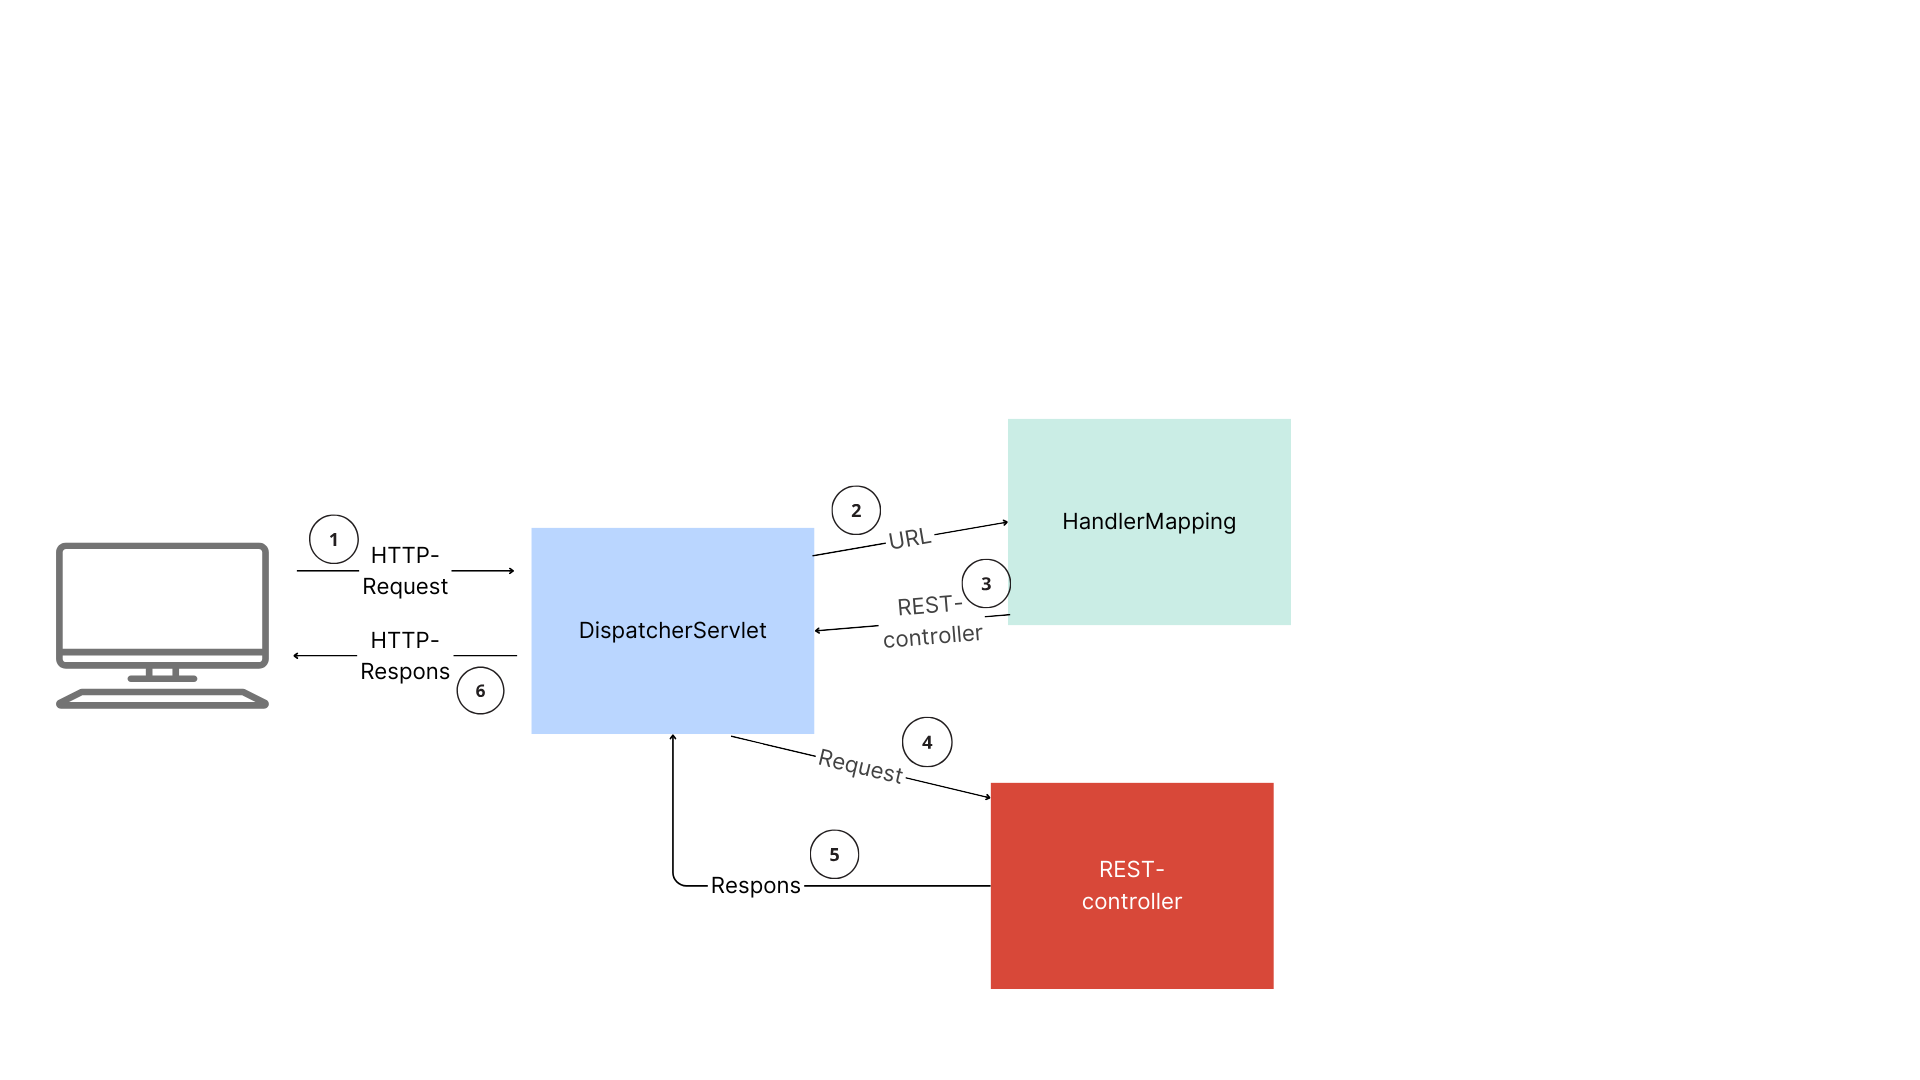
\includegraphics[width=\linewidth]{images/chapter-rest/dispatcherservlet.png}
  \caption{Een REST-verzoek afhandelen}
  \label{fig:test_passed}
\end{figure}

De component van Spring Boot die verantwoordelijk is dat een HTTP-request door de juiste REST-controller wordt afgehandeld is de DispatcherServlet.  De DispatcherServlet is onderdeel van Spring MVC.  De DispatcherServlet bepaalt welke controller een HTTP-request moet afhandelen,  hij geeft het request door aan de juiste controller en  verwerkt het respons van de controller om een HTTP-respons terug te sturen naar de client.

Om te achterhalen welke REST-controller verantwoordelijk is om een HTTP-request af te handelen raadpleegt de DispatcherServlet de HandlerMapping. De HandlerMapping is als het ware een kaart die URL's koppelt aan specifieke controllerklassen en methoden.
Op basis van de URL in het binnenkomende request bepaalt de DispatcherServlet welke controllerklasse en methode verantwoordelijk zijn voor het afhandelen van het request.


\begin{oefening}
Maak het package \textit{be.pxl.demo.api}.  Voeg de klasse \textbf{GreetingController} toe het package.  Start de Spring Boot applicatie en open de URL \url{http://localhost:8080/greetings/hello} in een browser. Voeg in de REST-controller een methode toe met de URI GET /greetings/daytime die de huidige dag en het tijdstip teruggeeft in het formaat 'Maandag 18 september 2023'.
\end{oefening}

\section{MusicPlaylist}

We gaan een nieuwe Spring Boot toepassing aanmaken waarmee we een muziek playlist beheren. 

\begin{oefening}
Maak een nieuwe Spring boot toepassing MusicPlaylist. We gebruiken Spring MVC om een RESTful web applicatie te maken.  
\end{oefening}

\subsection{Een liedje toevoegen aan een playlist}

\begin{apiRoute}{post}{/playlist/songs}{Add a new song to the playlist.}
\begin{routeRequest}{application/json}
\begin{routeRequestBody}
{
  "title": "Hello",
  "artist": "Adele",
  "duration_seconds": 293,
  "genre": "POP"
}
\end{routeRequestBody}
\end{routeRequest}
\begin{routeResponse}{application/json}
\begin{routeResponseItem}{200}{ok}
\end{routeResponseItem}
\end{routeResponse}
\end{apiRoute}


Om te beginnen hebben we de klasse Song nodig. 

\begin{lstlisting}[language=java,  frame=single]
public class Song {
    private String title;
    private String artist;
    @JsonProperty("duration_seconds")
    private int durationSeconds;
    private Genre genre;

    // Default constructor
    public Song() {
    }

    // Parameterized constructor
    public Song(String title, String artist, int durationSeconds, Genre genre) {
        this.title = title;
        this.artist = artist;
        this.durationSeconds = durationSeconds;
        this.genre = genre;
    }

    // Getter and setter methods
    public String getTitle() {
        return title;
    }

    public void setTitle(String title) {
        this.title = title;
    }

    public String getArtist() {
        return artist;
    }

    public void setArtist(String artist) {
        this.artist = artist;
    }

    public int getDurationSeconds() {
        return durationSeconds;
    }

    public void setDurationSeconds(int durationSeconds) {
        this.durationSeconds = durationSeconds;
    }

    public Genre getGenre() {
        return genre;
    }

    public void setGenre(Genre genre) {
        this.genre = genre;
    }

    @Override
    public String toString() {
        return "Song{" +
                "title='" + title + '\'' +
                ", artist='" + artist + '\'' +
                ", durationSeconds=" + durationSeconds +
                ", genre='" + genre + '\'' +
                '}';
    }
}
\end{lstlisting}


Nu gaan we de REST-controller implementeren.  We gaan hierin een methode voorzien die een POST op de URI /playlist/songs kan afhandelen.  Initieel gaan we enkel de titel in de loggegevens tonen. 

\begin{lstlisting}[language=java,  frame=single]
@RestController
@RequestMapping("/playlist/songs")
public class MusicPlaylistController {

	private static final Logger LOGGER = LoggerFactory.getLogger(MusicPlaylistController.class);

	@PostMapping
	public void addSong(@RequestBody Song song) {
		if (LOGGER.isInfoEnabled()) {
			LOGGER.info("Adding song [" + song.getTitle() + "]");
		}
	}
}
\end{lstlisting}

De liedjes die aan de playlist worden toegevoegd willen we bijhouden. Later zullen we ze wegschrijven in een databank, maar voorlopig gaan we ze bijhouden in een lijst.
Om dit mogelijk te maken gaan we een nieuwe Spring Bean toevoegen: de MusicPlaylistService.  

\begin{lstlisting}[language=java,  frame=single]
package be.pxl.demo;

import be.pxl.demo.domain.Song;
import org.springframework.stereotype.Service;

import java.util.ArrayList;
import java.util.List;

@Service
public class MusicPlaylistService {
	private final List<Song> myPlaylist = new ArrayList<>();

	public void addSong(Song song) {
		myPlaylist.add(song);
	}
}
\end{lstlisting}

De MusicPlaylistService wordt geannoteerd met @Service .
In onze Spring Boot applicaties gaan we steeds de business-logica implementeren in de service-laag.  De @Service annotatie wordt gebruikt voor de componenten (Spring Beans) in de service-laag.  Wanneer onze Spring Boot applicatie opstart wordt er exact \'e\'en instantie van de MusicPlaylistService aangemaakt in de ApplicationContext en deze instantie wordt tijdens de volledige levensduur van de toepassing gebruikt.  Dit noemen we de scope van de service en de default scope noemen we \textbf{singleton}. 
Dit betekent dat we \'e\'en enkele, gedeelde playlist hebben voor alle gebruikers.

Nu gaan we de MusicPlaylistService beschikbaar maken in de MusicPlaylistController.
We maken gebruik van \textbf{constructor injection}.  Zodra de instantie van de MusicPlaylistController door Spring Boot wordt aangemaakt, zal er eerst gezorgd worden dat de instantie MusicPlaylistService aangemaakt wordt. Deze instantie wordt dan achter de schermen meegegeven aan de constructor van de MusicPlaylistController. Zo kan ons MusicPlaylistController-object het MusicPlaylistService-object gebruiken.
Omdat er maar \'e\'en constructor is, is de annotatie @Autowired eigenlijk overbodig.

\begin{lstlisting}[language=java,  frame=single]
@RestController
@RequestMapping("/playlist/songs")
public class MusicPlaylistController {

	private static final Logger LOGGER = LoggerFactory.getLogger(MusicPlaylistController.class);
	private final MusicPlaylistService musicPlaylistService;

	@Autowired
	public MusicPlaylistController(MusicPlaylistService musicPlaylistService) {
		this.musicPlaylistService = musicPlaylistService;
	}

	@PostMapping
	public void addSong(@RequestBody Song song) {
		if (LOGGER.isInfoEnabled()) {
			LOGGER.info("Adding song [" + song.getTitle() + "]");
		}
		musicPlaylistService.addSong(song);
	}
}
\end{lstlisting}

Test nu het POST-verzoek.  Je kan Postman,  Insomnia of een andere tool gebruiken om een POST-verzoek naar de toepassing te sturen.  De toegevoegde liedjes gaan uiteraard verloren wanneer je de toepassing herstart. 

\begin{figure}[H]
  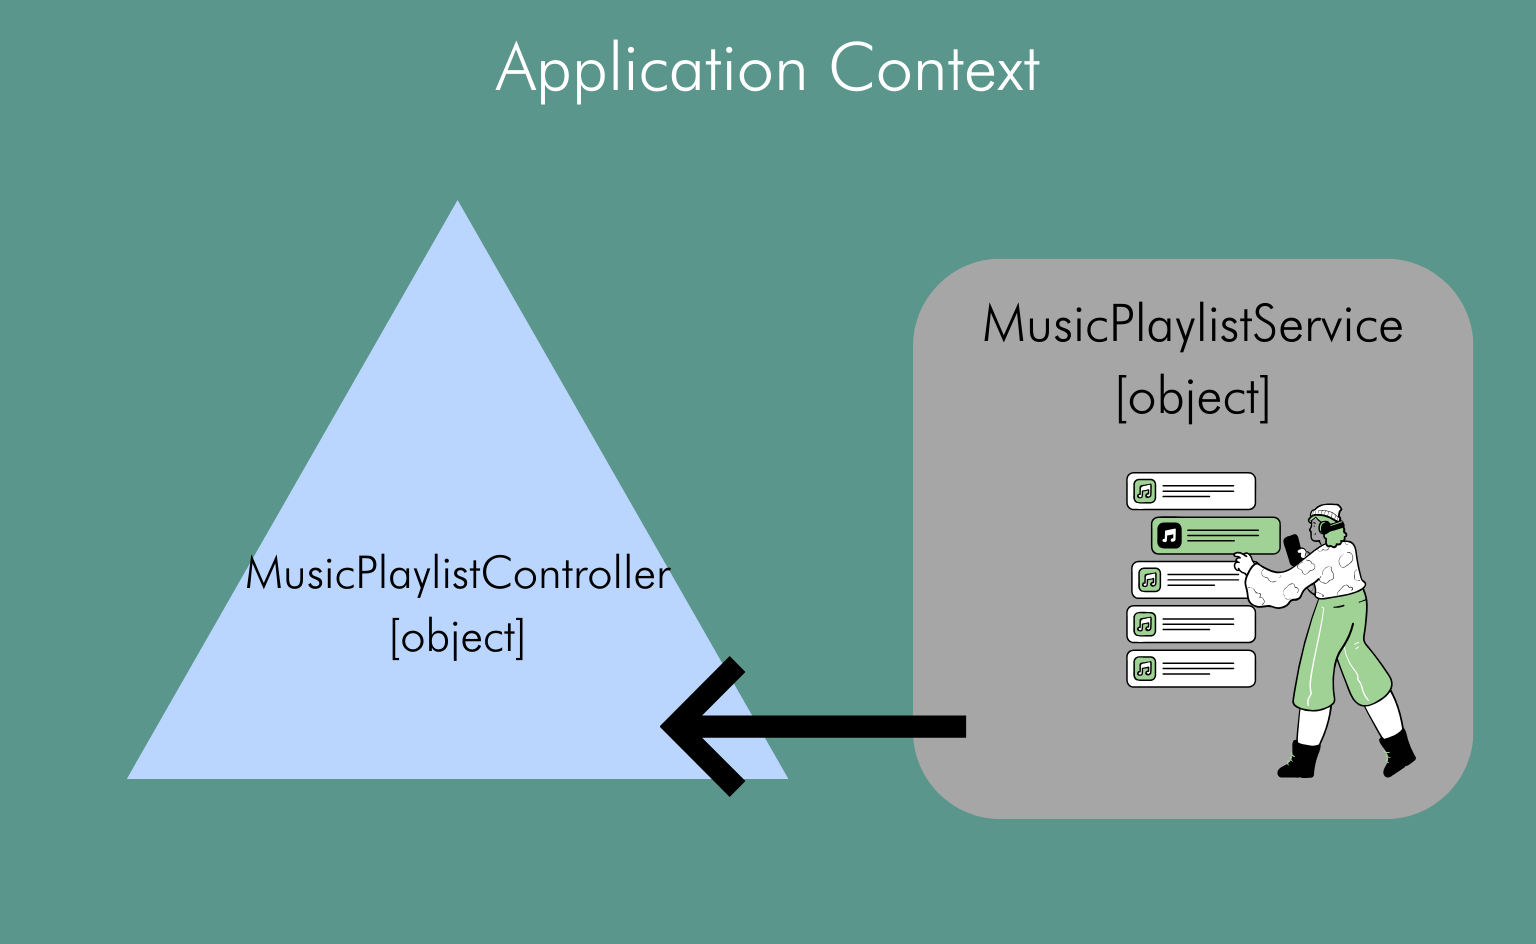
\includegraphics[width=\linewidth]{images/chapter-rest/applicationcontext_musicplaylist.png}
  \caption{Spring Beans in de Application Context}
  \label{fig:spring_beans_musicplaylist}
\end{figure}


\begin{figure}[H]
  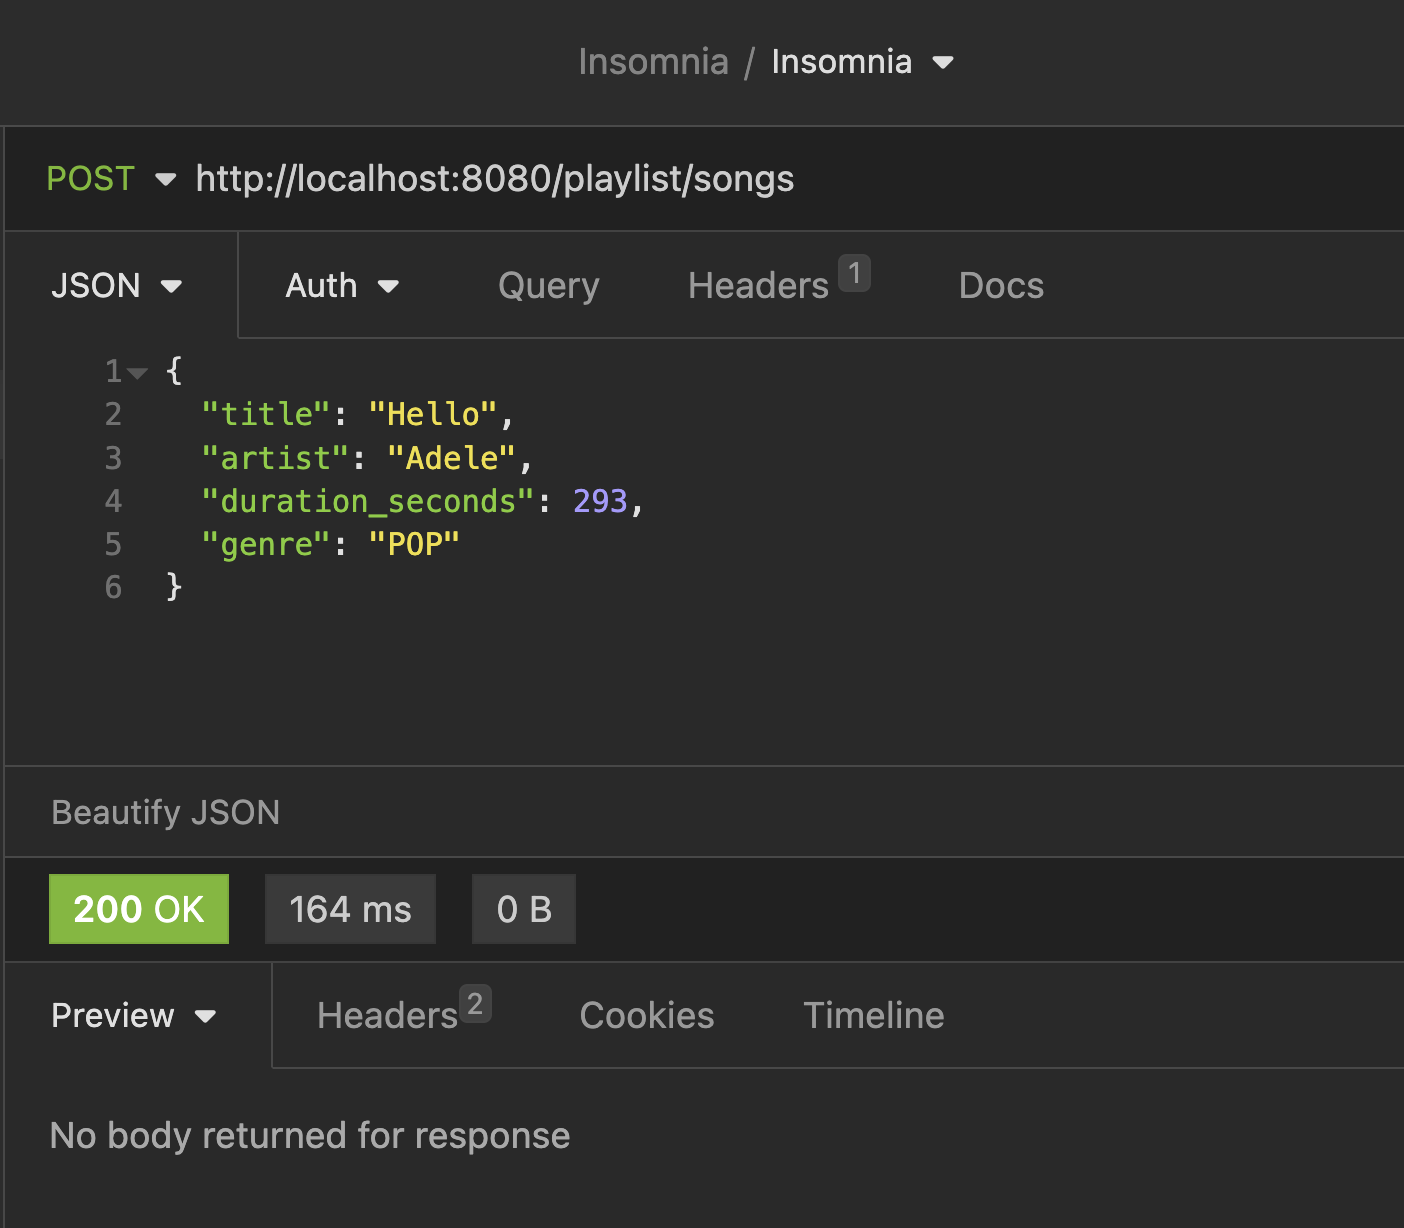
\includegraphics[width=\linewidth]{images/chapter-rest/insomnia_post.png}
  \caption{POST-verzoek met Insomnia}
  \label{fig:post_request}
\end{figure}

\subsection{De playlist opvragen}


\begin{apiRoute}{get}{/playlist/songs}{Retrieve all songs from the playlist}
\begin{routeParameter}
	\noRouteParameter {no parameter }
\end{routeParameter}
\begin{routeRequest}{application/json}
\end{routeRequest}
\begin{routeResponse}{application/json}
\begin{routeResponseItem}{200}{ok}
\begin{routeResponseItemBody}
[
	{
		"title": "Hello",
		"artist": "Adele",
		"genre": "POP",
		"duration_seconds": 293
	},
	{
		"title": "Shape of You",
		"artist": "Ed Sheeran",
		"genre": "POP",
		"duration_seconds": 233
	},
	{
		"title": "Umbrella",
		"artist": "Rihanna",
		"genre": "RNB",
		"duration_seconds": 264
	}
]
\end{routeResponseItemBody}
\end{routeResponseItem}
\end{routeResponse}
\end{apiRoute}


\begin{lstlisting}[language=java,  frame=single]
package be.pxl.demo;

import be.pxl.demo.domain.Song;
import org.springframework.stereotype.Service;

import java.util.ArrayList;
import java.util.List;

@Service
public class MusicPlaylistService {
	private final List<Song> myPlaylist = new ArrayList<>();

	public void addSong(Song song) {
		myPlaylist.add(song);
	}

	public List<Song> getSongs() {
		return myPlaylist;
	}
}
\end{lstlisting}


\begin{lstlisting}[language=java,  frame=single]
package be.pxl.demo.controller;

import be.pxl.demo.MusicPlaylistService;
import be.pxl.demo.domain.Song;
import org.slf4j.Logger;
import org.slf4j.LoggerFactory;
import org.springframework.beans.factory.annotation.Autowired;
import org.springframework.web.bind.annotation.GetMapping;
import org.springframework.web.bind.annotation.PostMapping;
import org.springframework.web.bind.annotation.RequestBody;
import org.springframework.web.bind.annotation.RequestMapping;
import org.springframework.web.bind.annotation.RestController;

import java.util.List;

@RestController
@RequestMapping("/playlist/songs")
public class MusicPlaylistController {

	private static final Logger LOGGER = LoggerFactory.getLogger(MusicPlaylistController.class);
	private final MusicPlaylistService musicPlaylistService;

	@Autowired
	public MusicPlaylistController(MusicPlaylistService musicPlaylistService) {
		this.musicPlaylistService = musicPlaylistService;
	}

	@PostMapping
	public void addSong(@RequestBody Song song) {
		if (LOGGER.isInfoEnabled()) {
			LOGGER.info("Adding song [" + song.getTitle() + "]");
		}
		musicPlaylistService.addSong(song);
	}

	@GetMapping
	public List<Song> getSongs() {
		return musicPlaylistService.getSongs();
	}
}
\end{lstlisting}

\subsection{Liedjes van \'e\'en genre}


 
 \begin{apiRoute}{get}{/playlist/songs/\{genre\}}{Retrieve all songs from the playlist with the given genre}
\begin{routeParameter}
	\routeParamItem{genre}{the requested genre}
\end{routeParameter}
\begin{routeRequest}{application/json}
\end{routeRequest}
\begin{routeResponse}{application/json}
\begin{routeResponseItem}{200}{ok}
\begin{routeResponseItemBody}
[
	{
		"title": "Hello",
		"artist": "Adele",
		"genre": "POP",
		"duration_seconds": 293
	},
	{
		"title": "Shape of You",
		"artist": "Ed Sheeran",
		"genre": "POP",
		"duration_seconds": 233
	}
]
\end{routeResponseItemBody}
\end{routeResponseItem}
\end{routeResponse}
\end{apiRoute}


\begin{lstlisting}[language=java,  frame=single]
package be.pxl.demo.controller;

import be.pxl.demo.MusicPlaylistService;
import be.pxl.demo.domain.Genre;
import be.pxl.demo.domain.Song;
import org.slf4j.Logger;
import org.slf4j.LoggerFactory;
import org.springframework.beans.factory.annotation.Autowired;
import org.springframework.web.bind.annotation.GetMapping;
import org.springframework.web.bind.annotation.PathVariable;
import org.springframework.web.bind.annotation.PostMapping;
import org.springframework.web.bind.annotation.RequestBody;
import org.springframework.web.bind.annotation.RequestMapping;
import org.springframework.web.bind.annotation.RestController;

import java.util.List;

@RestController
@RequestMapping("/playlist/songs")
public class MusicPlaylistController {

	private static final Logger LOGGER = LoggerFactory.getLogger(MusicPlaylistController.class);
	private final MusicPlaylistService musicPlaylistService;

	@Autowired
	public MusicPlaylistController(MusicPlaylistService musicPlaylistService) {
		this.musicPlaylistService = musicPlaylistService;
	}

	@PostMapping
	public void addSong(@RequestBody Song song) {
		if (LOGGER.isInfoEnabled()) {
			LOGGER.info("Adding song [" + song.getTitle() + "]");
		}
		musicPlaylistService.addSong(song);
	}

	@GetMapping
	public List<Song> getSongs() {
		return musicPlaylistService.getSongs();
	}

	@GetMapping("{genre}")
	public List<Song> getSongs(@PathVariable Genre genre) {
		return musicPlaylistService.getSongsByGenre(genre);
	}
}
\end{lstlisting}

\begin{lstlisting}[language=java,  frame=single]
package be.pxl.demo;

import be.pxl.demo.domain.Genre;
import be.pxl.demo.domain.Song;
import org.springframework.stereotype.Service;

import java.util.ArrayList;
import java.util.List;

@Service
public class MusicPlaylistService {
	private final List<Song> myPlaylist = new ArrayList<>();

	public void addSong(Song song) {
		myPlaylist.add(song);
	}

	public List<Song> getSongs() {
		return myPlaylist;
	}

	public List<Song> getSongsByGenre(Genre genre) {
		List<Song> response = new ArrayList<>();
		for (Song song : myPlaylist) {
			if (song.getGenre() == genre) {
				response.add(song);
			}
		}
		return response;
	}
}
\end{lstlisting}


\subsection{Gegevens van een liedje aanpassen}

Als je een nieuwe song in de playlist toevoegt, dan wordt deze steeds achteraan in de lijst toegevoegd. We kunnen nu de gegevens van het liedje op een gegeven positie in de lijst gaan overschrijven of aanpassen.  De index die we meegeven is een waarde van 0 tot 1 minder dan de lengte van de lijst.  Later zullen we zien hoe we een duidelijke foutboodschap kunnen geven aan de client als een foutieve index-waarde wordt gegeven.

Om de gegevens van een liedje aan te passen gebruiken we een PUT-verzoek. 
Je moet steeds alle gegevens van het liedje meegeven in de requestbody. 

\begin{apiRoute}{put}{/musicplaylist/songs\{index\}}{Update the song at the given index.}
\begin{routeParameter}
\routeParamItem{code}{unique identification of a house}
\end{routeParameter}
\begin{routeRequest}{application/json}
\begin{routeRequestBody}
{
		"title": "Hello",
		"artist": "Adele",
		"genre": "POP",
		"duration_seconds": 293
}
\end{routeRequestBody}
\end{routeRequest}
\begin{routeResponse}{application/json}
\begin{routeResponseItem}{200}{ok}
\end{routeResponseItem}
\end{routeResponse}
\end{apiRoute}


\begin{lstlisting}
package be.pxl.demo.controller;

import be.pxl.demo.MusicPlaylistService;
import be.pxl.demo.domain.Genre;
import be.pxl.demo.domain.Song;
import org.slf4j.Logger;
import org.slf4j.LoggerFactory;
import org.springframework.beans.factory.annotation.Autowired;
import org.springframework.web.bind.annotation.DeleteMapping;
import org.springframework.web.bind.annotation.GetMapping;
import org.springframework.web.bind.annotation.PathVariable;
import org.springframework.web.bind.annotation.PostMapping;
import org.springframework.web.bind.annotation.PutMapping;
import org.springframework.web.bind.annotation.RequestBody;
import org.springframework.web.bind.annotation.RequestMapping;
import org.springframework.web.bind.annotation.RestController;

import java.util.List;

@RestController
@RequestMapping("/playlist/songs")
public class MusicPlaylistController {

	private static final Logger LOGGER = LoggerFactory.getLogger(MusicPlaylistController.class);
	private final MusicPlaylistService musicPlaylistService;

	@Autowired
	public MusicPlaylistController(MusicPlaylistService musicPlaylistService) {
		this.musicPlaylistService = musicPlaylistService;
	}

	@PostMapping
	public void addSong(@RequestBody Song song) {
		if (LOGGER.isInfoEnabled()) {
			LOGGER.info("Adding song [" + song.getTitle() + "]");
		}
		musicPlaylistService.addSong(song);
	}

	@GetMapping
	public List<Song> getSongs() {
		return musicPlaylistService.getSongs();
	}

	@GetMapping("/{genre}")
	public List<Song> getSongs(@PathVariable Genre genre) {
		return musicPlaylistService.getSongsByGenre(genre);
	}

	@PutMapping("/{index}")
	public void updateSong(@PathVariable int index, @RequestBody Song song) {
		musicPlaylistService.updateSong(index, song);
	}
}
\end{lstlisting}

\begin{lstlisting}
package be.pxl.demo;

import be.pxl.demo.domain.Genre;
import be.pxl.demo.domain.Song;
import org.springframework.stereotype.Service;

import java.util.ArrayList;
import java.util.List;

@Service
public class MusicPlaylistService {
	private final List<Song> myPlaylist = new ArrayList<>();

	public void addSong(Song song) {
		myPlaylist.add(song);
	}

	public List<Song> getSongs() {
		return myPlaylist;
	}

	public List<Song> getSongsByGenre(Genre genre) {
		List<Song> response = new ArrayList<>();
		for (Song song : myPlaylist) {
			if (song.getGenre() == genre) {
				response.add(song);
			}
		}
		return response;
	}

	public void updateSong(int index, Song song) {
		myPlaylist.set(index, song);
	}

	public void deleteSong(int index) {
		myPlaylist.remove(index);
	}
}
\end{lstlisting}

We vervangen het liedje op de opgegeven index door een nieuw Song-object met de aangepaste gegevens.

\subsection{Een liedje verwijderen}

Om een liedje op een opgegeven index uit de playlist te verwijderen gaan we een DELETE-verzoek implementeren.


\begin{apiRoute}{delete}{/musicplaylist/songs/\{index\}}{Delete the song at the given index.}
\begin{routeParameter}
\routeParamItem{index}{position of the song to be deleted}
\end{routeParameter}
\begin{routeResponse}{application/json}
\begin{routeResponseItem}{200}{ok}
\end{routeResponseItem}
\end{routeResponse}
\end{apiRoute}

\begin{lstlisting}
package be.pxl.demo.controller;

import be.pxl.demo.MusicPlaylistService;
import be.pxl.demo.domain.Genre;
import be.pxl.demo.domain.Song;
import org.slf4j.Logger;
import org.slf4j.LoggerFactory;
import org.springframework.beans.factory.annotation.Autowired;
import org.springframework.web.bind.annotation.DeleteMapping;
import org.springframework.web.bind.annotation.GetMapping;
import org.springframework.web.bind.annotation.PathVariable;
import org.springframework.web.bind.annotation.PostMapping;
import org.springframework.web.bind.annotation.PutMapping;
import org.springframework.web.bind.annotation.RequestBody;
import org.springframework.web.bind.annotation.RequestMapping;
import org.springframework.web.bind.annotation.RestController;

import java.util.List;

@RestController
@RequestMapping("/playlist/songs")
public class MusicPlaylistController {

	private static final Logger LOGGER = LoggerFactory.getLogger(MusicPlaylistController.class);
	private final MusicPlaylistService musicPlaylistService;

	@Autowired
	public MusicPlaylistController(MusicPlaylistService musicPlaylistService) {
		this.musicPlaylistService = musicPlaylistService;
	}

	@PostMapping
	public void addSong(@RequestBody Song song) {
		if (LOGGER.isInfoEnabled()) {
			LOGGER.info("Adding song [" + song.getTitle() + "]");
		}
		musicPlaylistService.addSong(song);
	}

	@GetMapping
	public List<Song> getSongs() {
		return musicPlaylistService.getSongs();
	}

	@GetMapping("/{genre}")
	public List<Song> getSongs(@PathVariable Genre genre) {
		return musicPlaylistService.getSongsByGenre(genre);
	}

	@PutMapping("/{index}")
	public void updateSong(@PathVariable int index, @RequestBody Song song) {
		musicPlaylistService.updateSong(index, song);
	}

	@DeleteMapping("/{index}")
	public void updateSong(@PathVariable int index) {
		musicPlaylistService.deleteSong(index);
	}
}
\end{lstlisting}


\begin{lstlisting}
package be.pxl.demo;

import be.pxl.demo.domain.Genre;
import be.pxl.demo.domain.Song;
import org.springframework.stereotype.Service;

import java.util.ArrayList;
import java.util.List;

@Service
public class MusicPlaylistService {
	private final List<Song> myPlaylist = new ArrayList<>();

	public void addSong(Song song) {
		myPlaylist.add(song);
	}

	public List<Song> getSongs() {
		return myPlaylist;
	}

	public List<Song> getSongsByGenre(Genre genre) {
		List<Song> response = new ArrayList<>();
		for (Song song : myPlaylist) {
			if (song.getGenre() == genre) {
				response.add(song);
			}
		}
		return response;
	}

	public void updateSong(int index, Song song) {
		myPlaylist.set(index, song);
	}

	public void deleteSong(int index) {
		myPlaylist.remove(index);
	}
}
\end{lstlisting}


\begin{oefening}\textbf{Huizenjacht}
We maken een Spring Boot toepassing om het aanbod op de huizenmarkt te beheren.
Ontwikkel een RESTful web toepassing met onderstaande endpoints.
Je voorziet een component HouseService met \'e\'en enkele, gedeelde lijst van woningen  voor alle gebruikers.

Een huis wordt voorgesteld als een resource met volgende eigenschappen:

\begin{itemize}
  \item \texttt{code} (string): Unieke identificatie van het huis.
  \item \texttt{name} (string): Naam of beschrijving van het huis.
  \item \texttt{status} (enum): Status FOR\_SALE of SOLD.
  \item \texttt{city} (string): Locatie van het huis.
  \item \texttt{price} (double): Prijs van het huis.
\end{itemize}

\section{REST Endpoints}

\begin{apiRoute}{post}{/houses}{Create a new house.}
\begin{routeParameter}
	\noRouteParameter {no parameter }
\end{routeParameter}
\begin{routeRequest}{application/json}
\begin{routeRequestBody}
{
  "code": "HAS_001",
  "name": "Beautiful house in the city",
  "city": "Hasselt",
  "price": 250000
}
\end{routeRequestBody}
\end{routeRequest}
\begin{routeResponse}{application/json}
\begin{routeResponseItem}{200}{ok}
\end{routeResponseItem}
\end{routeResponse}
\end{apiRoute}


\begin{apiRoute}{put}{/houses/\{code\}}{Update the data (status, price,...) of the house with the given code.}
\begin{routeParameter}
\routeParamItem{code}{unique identification of a house}
\end{routeParameter}
\begin{routeRequest}{application/json}
\begin{routeRequestBody}
{
  "status": "SOLD"
  "name": "Beautiful house in the city",
  "price": 320000
}
\end{routeRequestBody}
\end{routeRequest}
\begin{routeResponse}{application/json}
\begin{routeResponseItem}{200}{ok}
\end{routeResponseItem}
\end{routeResponse}
\end{apiRoute}

\begin{apiRoute}{get}{/houses}{Retrieve all houses.}
\begin{routeParameter}
	\noRouteParameter {no parameter }
\end{routeParameter}
\begin{routeResponse}{application/json}
\begin{routeResponseItem}{200}{ok}
\begin{routeResponseItemBody}
[
  {
    "code": "GNK_001",
    "name": "Beautiful house in the city",
    "status": "SOLD",
     "city": "Genk",
    "price": 250000
  },
  {
    "code": "HAS_003",
    "name": "Cozy bungalow",
    "status": "FOR_SALE",
     "city": "Hasselt",
    "price": 180000
  }
]
\end{routeResponseItemBody}
\end{routeResponseItem}
\end{routeResponse}
\end{apiRoute}

\begin{apiRoute}{delete}{/houses/\{code\}}{Delete the house with the given code.}
\begin{routeParameter}
\routeParamItem{code}{unique identification of a house}
\end{routeParameter}
\begin{routeResponse}{application/json}
\begin{routeResponseItem}{200}{ok}
\end{routeResponseItem}
\end{routeResponse}
\end{apiRoute}

\end{oefening}

\chapter{Foutafhandeling}

\begin{summary}
Tijdens het uitvoeren van een programma kan en zal er vanalles foutgaan. De gebruiker van het programma geeft de datum in in een foutief formaat, een printer is offline, er is onvoldoende schrijfruimte vrij om een bestand weg te schrijven, het programma kreeg onvoldoende geheugen toegewezen,... Fouten die zich voordoen tijdens het uitvoeren van een programma, at runtime dus, verdelen we onder in errors en exceptions. Errors zijn de fouten die meestal veroorzaakt worden door het onderliggende besturingssysteem. Tijdens het verloop van het programma kunnen deze errors niet meer opgelost worden en het programma zal daarom be\"eindigd worden. Dit is niet het geval voor exceptions. Je kan je code op een defensieve manier schrijven en rekening houden met de mogelijke exceptions die kunnen optreden. ``Exception handling'' is het proces om deze exceptions op een correcte en liefst gebruiksvriendelijke manier af te handelen. Indien een fout niet correct wordt afgehandeld, zal het programma alsnog voortijdig afgebroken worden, maar met de juiste foutafhandeling kan de uitvoer van het programma gewoon verdergezet worden. 
 \end{summary}
 
\section{Compile-time vs runtime errors}

Een programmeur schrijft Java code in zijn editor of favoriete IDE. Vervolgens wordt de Java code gecompileerd tot bytecode. Deze bytecode wordt door de JVM (Java Virtual Machine) ge\"interpreteerd tot machinecode instructies die worden uitgevoerd door het computersysteem.

Wanneer dus een Java programma wordt opgestart, kunnen er 2 categorie\"en van problemen voorkomen. Het kan zijn dat het Java programma niet gecompileerd kan worden. In dat geval spreken we van een compile-time error. Indien het programma succesvol gecompileerd wordt, kan er zich tijdens het uitvoeren van de code een probleem voordoen, in dat geval spreken we van runtime errors of exceptions. 

\begin{figure}[H]
  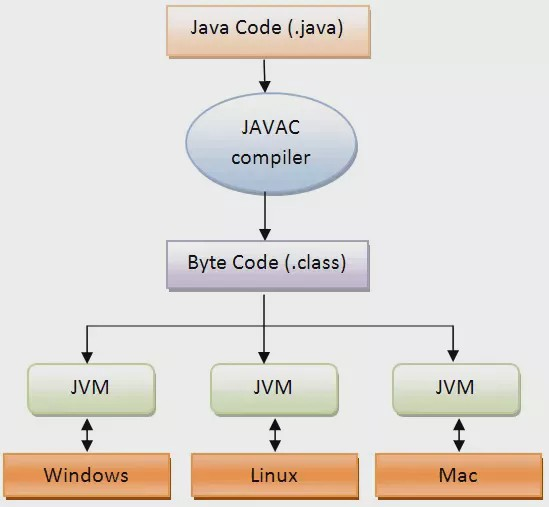
\includegraphics[width=\linewidth]{images/h1/java_compiler.jpeg}
  \caption{Compiler, interpreter en Java Virtual Machine.}
  \label{fig:compiler}
\end{figure}


\begin{figure}[H]
  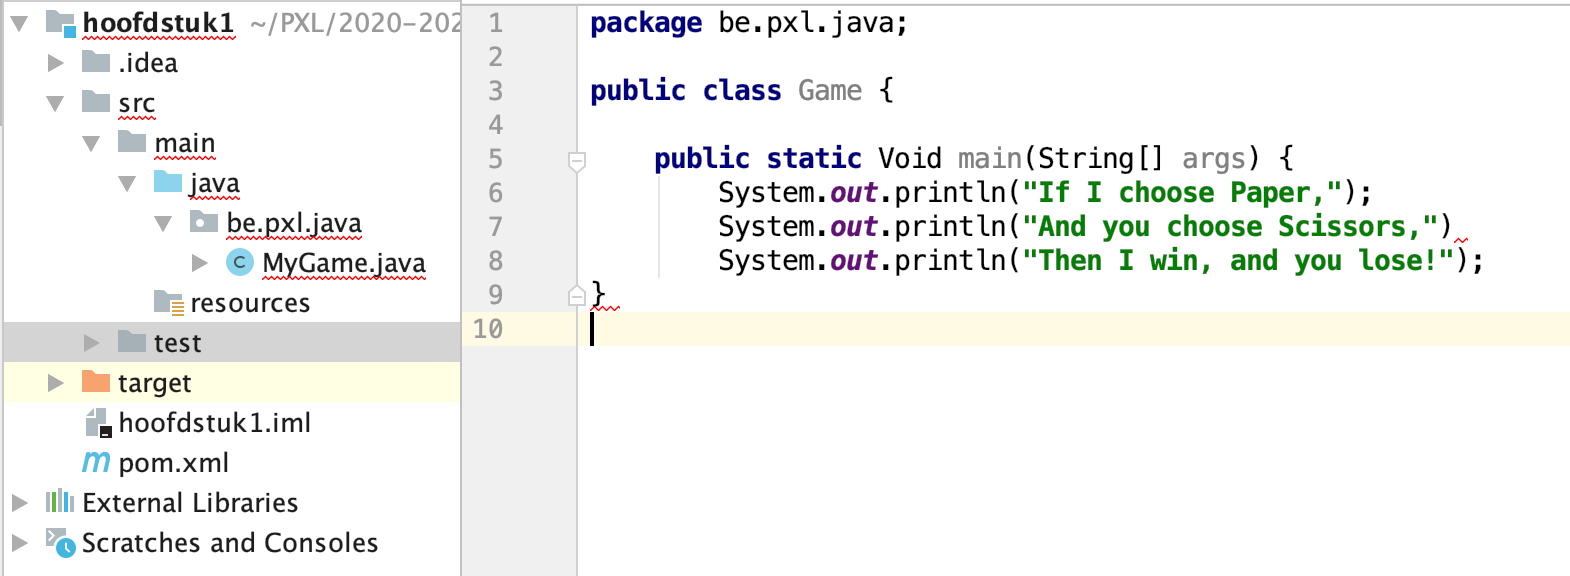
\includegraphics[width=\linewidth]{images/h1/compiletime_errors.png}
  \caption{Compile-time errors}
  \label{fig:compiletime_errors}
\end{figure}

\begin{oefening}
Welke compile-time errors kan je ontdekken in het volgende codefragment in figuur \ref{fig:compiletime_errors}?
\end{oefening}

Omdat Java een object-ge\"orienteerde programmeertaal is, wordt er ook een object gebruikt om aan te geven dat er iets fout ging bij uitvoeren van het Java programma. Zodra er zich een probleem voordoet tijdens het uitvoeren van een programma-instructie, wordt er een exception-object aangemaakt en ``opgeworpen''. Hierdoor stopt de normale uitvoer van het programma. Er wordt nog geprobeerd om het exception-object op een keurige manier af te handelen (indien die code aanwezig is), maar als dat niet lukt zal het programma be\"eindigd worden. Het exception-object bevat nuttige informatie voor de ontwikkelaar zoals de methode en lijn-nummer waar de exception werd aangemaakt en het type van de exception. 

\section{First catch}

\begin{lstlisting}
public class DivisionByZero {

	public static void main(String[] args) {
		int a = (1 + 1) % 2;
		int b = 5;
		int c = b / a;
		System.out.println("Het resultaat is " + c);
	}
}
\end{lstlisting}

Als je het bovenstaande programma uitvoert zal het volgende in de console verschijnen:

\begin{verbatim}
Exception in thread "main" java.lang.ArithmeticException: / by zero
	at be.pxl.ja.DivisionByZero.main(DivisionByZero.java:6)<5 internal calls>
\end{verbatim}
  
De variabele \textit{a} bevat inderdaad de waarde 0 en hierdoor hebben we dus te maken met een deling door 0. Zodra de deling wordt uitgevoerd loopt het dus fout en gooit de java runtime een ArithmeticException op. Omdat de ArithmeticException nergens wordt afgehandeld eindigt het programma. Je zal enkel nog een stacktrace zien verschijnen in de console. Een stacktrace is de naam en foutboodschap van de exception gevolgd door de weg die de exception heeft afgelegd (doorheen de methoden van je klassen) vanaf het moment dat ze werd opgegooid. We zien dus dat de exception is veroorzaakt op regel 6 in de klasse DivisionByZero.

\begin{lstlisting}
public class DivisionByZero {

	public static void main(String[] args) {
		int a = (1 + 1) % 2;
		int b = 5;
		try {
			int c = b / a;
			System.out.println("Het resultaat is " + c);
		} catch (ArithmeticException e) {
			System.out.println("You should not divide a number by zero.");
		}
		System.out.println("First catch completed!");
	}
}
\end{lstlisting}

\begin{verbatim}
You should not divide a number by zero.
First catch completed!
\end{verbatim}

We hebben de instructie met de deling nu in een try-blok geplaatst. Omdat de variabele c in het try-blok wordt aangemaakt, kan deze variabele ook enkel binnen het try-blok gebruikt worden. Indien een exception optreedt binnen een try-blok zal de programma-uitvoer de resterende code binnen het try-blok overslaan en verdergaan bij het eerste catch-blok dat direct volgt achter het try-blok. Je bent als programmeur verplicht om een try-blok steeds te laten volgen door \'e\'en of meerdere catch-blokken.
In het catch-blok wordt dan de code uitgevoerd om het probleem op te lossen of tenminste een duidelijke boodschap voor de gebruiker van het programma te voorzien.
Als alle instructies uit het catch-blok zijn uitgevoerd zal het programma zijn normale uitvoer verderzetten.


\section{Java exception hi\"erarchie}
  
\begin{figure}[H]
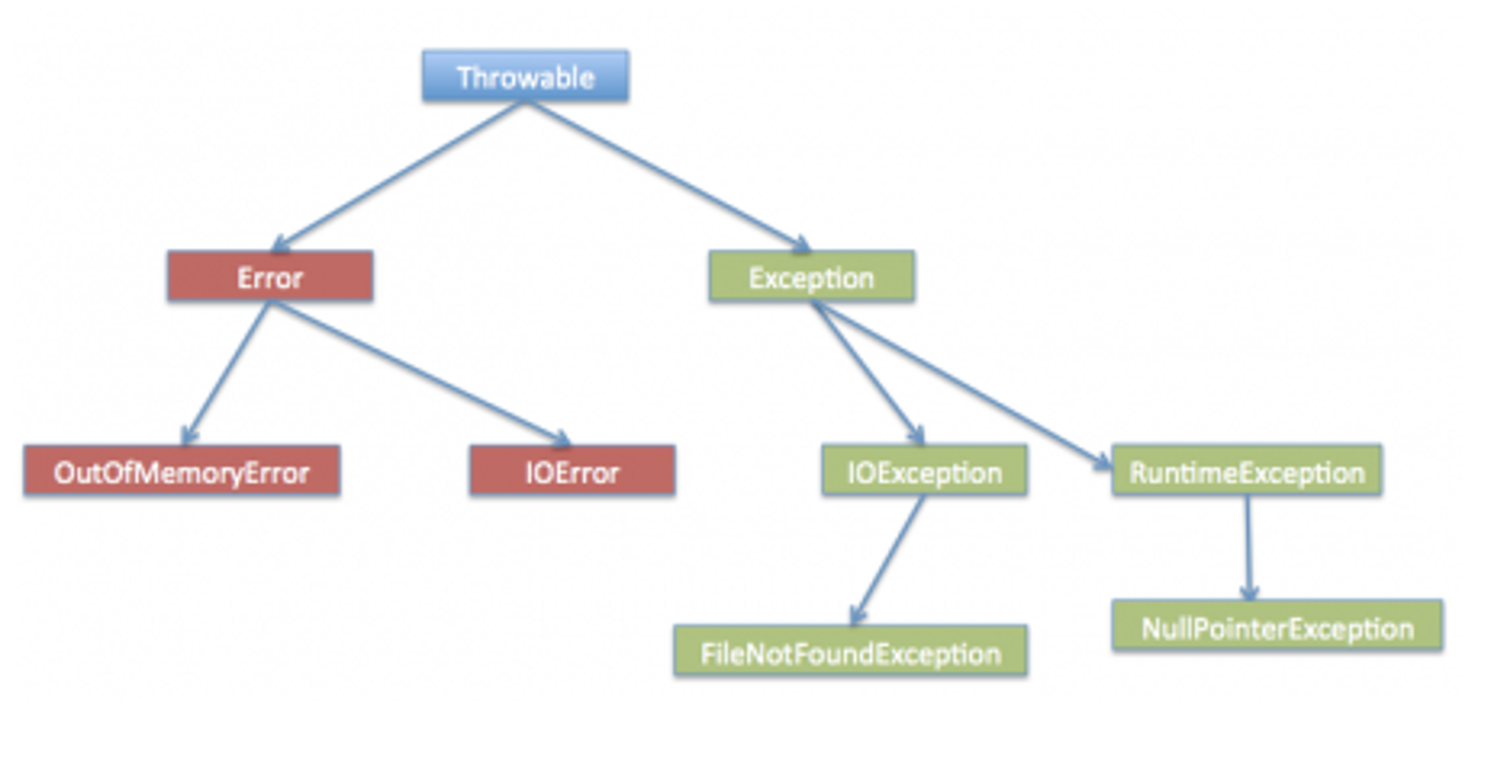
\includegraphics[width=\linewidth]{images/h1/exception-hierarchy.png}
\caption{Exception hi\"erarchie}
\label{fig:exceptiono_hierarchy}
\end{figure}
  
Zoals reeds vermeld wordt er een exception-object aangemaakt zodra zich een probleem voordoet in de code. 
Er is in Java een hi\"erarchie gebouwd van exception-klassen om verschillende soorten fouten in een programma te categorizeren. Throwable is de superklasse van alle exceptions en errors in Java. Er zijn dus 2 afgeleide klassen van Throwable: Error and Exception. Exceptions zijn nog verder onderverdeeld in \textbf{checked exceptions} en \textbf{runtime exceptions}.

\subsection{Errors}

Errors zijn problemen die zich voordoen tijdens het uitvoeren van het programma en die meestal niet gerelateerd zijn aan het programma zelf. Daarom is het onmogelijk om erop te anticiperen en te herstellen van deze fouten. Dit kan gaan van hardware falen, over JVM crashes en out of memory errors. We hebben een aparte hi\"erarchie van errors en we zullen nooit code toevoegen in ons programma om deze fouten af te handelen. We tonen hier enkel voorbeelden van errors.


\subsubsection{StackOverflowError}
Je hebt ongetwijfeld al eens per ongeluk een programma geschreven met een oneindige lus. 

\begin{lstlisting}
public class DemoStackOverflow {

	private static void printNumber(int x) {
		System.out.println(x);
		printNumber(x + 2);
	}

	public static void main(String[] args) {
		printNumber(15);
	}
}
\end{lstlisting}

\begin{verbatim}
15
17
19
...
36597
36599
Exception in thread "main" java.lang.StackOverflowError
	...
	at be.pxl.ja.DemoStackOverflow.printNumber(DemoStackOverflow.java:5)
	at be.pxl.ja.DemoStackOverflow.printNumber(DemoStackOverflow.java:5) 
	at be.pxl.ja.DemoStackOverflow.printNumber(DemoStackOverflow.java:5) 
	at be.pxl.ja.DemoStackOverflow.printNumber(DemoStackOverflow.java:5) 
	...
\end{verbatim}

De call stack is de manier waarop tijdens de uitvoer van een programma o.a. wordt bijgehouden welke functies worden aangeroepen. Wanneer je programma-uitvoer in een oneindige lus terechtkomt, stapelen de gegevens in de call stack zich razendsnel op en loopt de call stack vol. Het programma zal uiteindelijk eindigen met een StackOverflowError.

\begin{figure}[H]
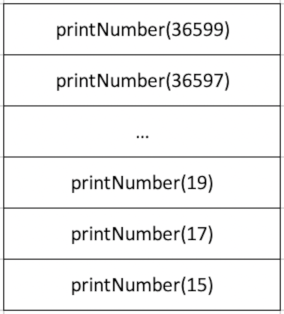
\includegraphics{images/h2/java_call_stack.png}
\caption{Java call stack}
\label{fig:call_stack}
\end{figure}


\subsubsection{OutOfMemoryError}

\begin{lstlisting}
public class DemoOutOfMemory {

	private void generateOutOfMemory() {
		Long maxMemory = Runtime.getRuntime().maxMemory();
		System.out.println(maxMemory);

		int[] matrix = new int[(int) (maxMemory + 1)];
		for (int i = 0; i < matrix.length; ++i) {
			matrix[i] = i + 1;
		}
		System.out.println("Matrix filled" + matrix[(int)(Math.random() * 100)]);

	}

	public static void main(String[] args) {
		DemoOutOfMemory doom = new DemoOutOfMemory();
		doom.generateOutOfMemory();
	}
}
\end{lstlisting}

Om de OutOfMemoryError te illustreren maken we een array aan die meer geheugenplaatsen inneemt dan de ruimte die het java programma ter beschikking heeft.

Als je dit programma uitvoert, pas je best het beschikbare geheugen voor het programma aan. Dit doe je door een waarde voor de VM optie -Xmx mee te geven.

\begin{itemize}
\item -Xmssize: Geeft de initi\"ele waarde voor de heap size.
\item -Xmxsize: Geeft de maximale waarde voor heap size.
\end{itemize}

De heap size van een Java programma is de hoeveelheid geheugen dat een Java-programma mag gebruiken om objecten op te slaan.

\begin{verbatim}
67108864
Exception in thread "main" java.lang.OutOfMemoryError: Java heap space
	at be.pxl.ja.DemoOutOfMemory.generateOutOfMemory(DemoOutOfMemory.java:8)
	at be.pxl.ja.DemoOutOfMemory.main(DemoOutOfMemory.java:16)<5 internal calls>
\end{verbatim}
	
\begin{figure}[H]
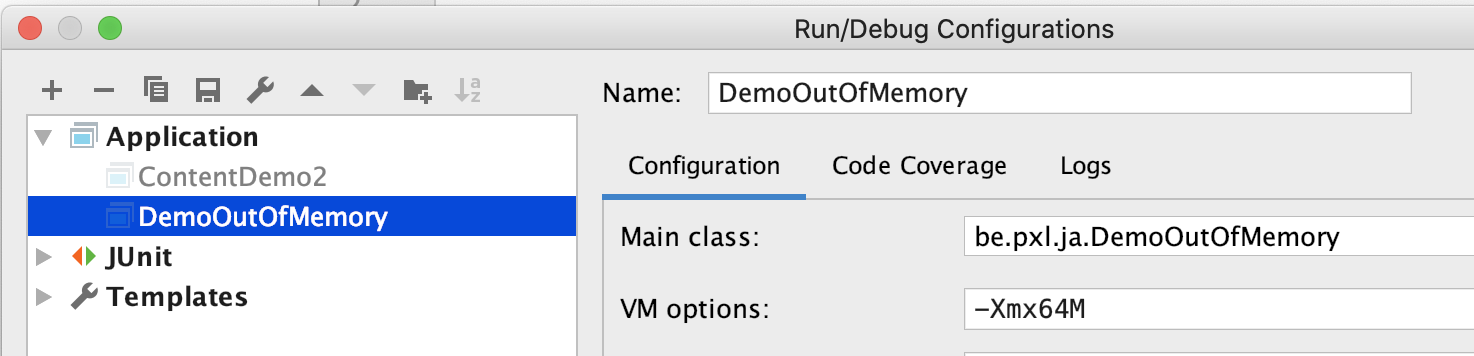
\includegraphics[width=\linewidth]{images/h2/jvm_options_xmx.png}
\caption{Maximum heap size aanpassen}
\label{fig:exceptiono_hierarchy}
\end{figure}

\subsection{Runtime exceptions}

Runtime exceptions zijn exceptions die vaak veroorzaakt worden door logische fouten in het programma.Typische voorbeelden van runtime exceptions zijn ArrayIndexOutOfBoundsException, NullPointerException en IllegalArgumentException. Vaak moet je ze niet afhandelen, maar moet je ervoor zorgen dat je de bug in je code oplost. Ook hier zijn onze unit testen heel belangrijk. Door goede unit testen te schrijven ga je runtime exceptions in je code opmerken en kunnen oplossen.

\begin{lstlisting}
public class Demo {

	public static void main(String[] args) {
		String tekst = "abc";
		System.out.println(tekst.repeat(-5));
	}
}
\end{lstlisting}

\begin{verbatim}
Exception in thread "main" java.lang.IllegalArgumentException: count is negative: -5
	at java.base/java.lang.String.repeat(String.java:3586)
	at be.pxl.ja.streamingservice.Demo.main(Demo.java:5)
\end{verbatim}

\begin{oefening}

\begin{lstlisting}
public class StreamingService {

	private List<Account> accounts;

	public void addAccount(Account account) {
		accounts.add(account);
	}
}
\end{lstlisting}

Welke exception doet zich voor zodra je voor een object van de klasse StreamingService de methode addAccount() aanroept? Waarom treedt die exception op?
\end{oefening}

Wanneer je programma gebruikmaakt van gegevens die door de gebruiker worden ingevoerd, moet je er altijd rekening mee houden dat de gebruiker foutieve gegevens kan ingeven. Deze foutieve gegevens kunnen aanleiding geven tot runtime exceptions. Ook hier moet je steeds anticiperen op de mogelijke input die de gebruiker kan invoeren. 


\begin{lstlisting}
public class ElementInArray {

	public static void main(String[] args) {
		String[] elements = { "H", "He", "Li", "Be", "B", "C", "N", "O", "F", "Ne" };

		Scanner scanner = new Scanner(System.in);
		
		// OPLOSSING 1
		System.out.println("Kies een nummer: ");
		int chosen = scanner.nextInt();
		if (chosen < elements.length) {
			System.out.println(elements[chosen]);
		} else {
			System.out.println("U koos een verkeerd nummer.");
		}

	    // OPLOSSING 2
		System.out.println("Kies een nummer: ");
		chosen = scanner.nextInt();
		try {
			System.out.println(elements[chosen]);
		} catch (ArrayIndexOutOfBoundsException e) {
			System.out.println("U koos een verkeerd nummer.");
		}
	}
}
\end{lstlisting}

In bovenstaand codevoorbeeld gaat onze voorkeur uit naar oplossing 1 waarbij de ingevoerde waarde wordt gecontroleerd vooraleer het element uit de array wordt benaderd. Deze code is makkelijker leesbaar en onderhoudbaar.

\begin{oefening}
Maak een programma dat de geboortedatum vraagt als input. Vervolgens berekent het programma hoeveel dagen het nog duurt vooraleer je jarig bent. Gebruik de methode parse() uit de klasse LocalDateTime om van de input van de gebruiker een LocalDateTime-object te maken. Welke exception kan optreden? Blijf input vragen totdat de gebruiker een correcte datum heeft ingegeven.
\end{oefening}


\subsection{Checked exceptions}

Wanneer je in java een methode aanroept, kan het voorkomen dat je direct een compileerfout voorgeschoteld krijgt. Het kan namelijk zijn dat java reeds anticipeert op mogelijke problemen en je dwingt om rekening te houden met het scenario dat er iets mis kan gaan. De compileerfout raakt pas opgelost wanneer je het afhandelen van de exception netjes programmeert.

Kijk eens naar onderstaand voorbeeld uit de streaming service.
We gebruiken hier de klasse MessageDigest uit JDK. Message digests zijn functies waarmee we voor input-data van willekeurige lengte een hash-waarde met een vaste lengte kunnen berekenen.  Als je de hash-waarde kent, kan je hieruit de input-data niet afleiden. We gebruiken dit om een paswoord bij te houden in een Account-object. We willen absoluut vermijden dat paswoorden in een leesbaar formaat in onze objecten worden bijgehouden.

Om een message digest te berekenen in Java moet je eerst de static methode getInstance() aanroepen met als parameter het door jouw gekozen algoritme. In dit voorbeeld wordt er gekozen voor MD5. Je ziet dat de lijn code, ondanks het feit dat alles correct is geschreven, toch rood wordt onderlijnd. Dat komt omdat de methode getInstance() een exception kan opgooien die we verplicht moeten afhandelen.

\begin{oefening}
Open de documentatie van de klasse MessageDigest en bekijk de uitleg voor de static methode getInstance(). Kan je hier zien welke exceptions er kunnen voorkomen?
\end{oefening}

\begin{figure}[H]
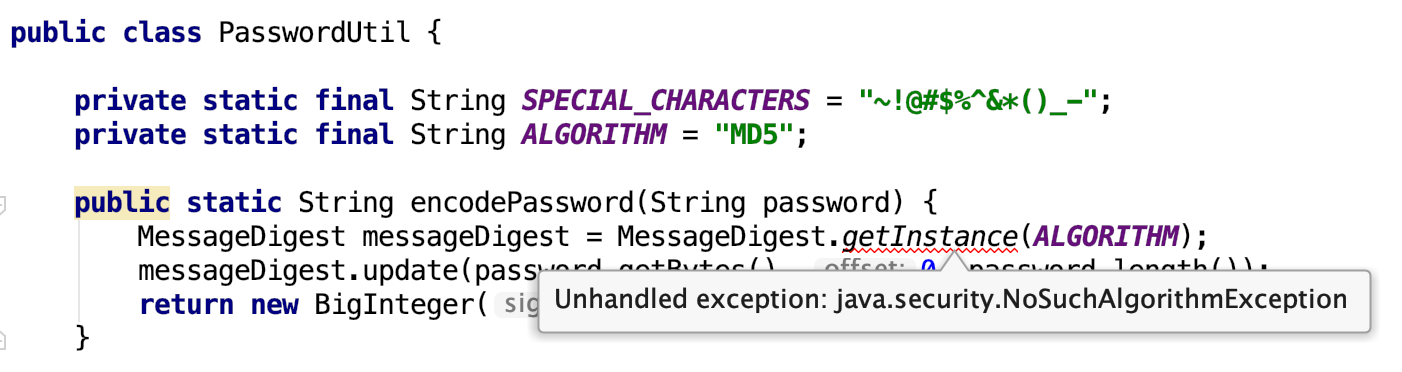
\includegraphics[width=\linewidth]{images/h2/no_such_algorithm_exception.png}
\caption{Een checked exception: NoSuchAlgorithmException}
\label{fig:no_such_algorithm}
\end{figure}

Deze compileerfout wordt veroorzaakt omdat de exception-klasse NoSuchAlgorithmException een checked exception is. Dit betekent dat het aanroepen van de methode die de exception gooit een compileerfout zal geven, omdat er geen code is toegevoegd om correct met de  exception om te gaan.
Er zijn 2 mogelijke oplossingen om deze compileerfout aan te pakken. Ofwel vang de exception op en handel je ze af in de methode encodePassword(), ofwel voeg je in de signatuur van de methode encodePassword() toe dat je de methode toelaat om een NoSuchAlgorithmException op te werpen. We geven nu eerst een voorbeeld van hoe je de exception kan opvangen en afhandelen. 

\begin{lstlisting}
import be.pxl.ja.streamingservice.util.PasswordUtil;

public class Account {
	private String email;
	private String password;

	public Account(String email, String password) {
		this.email = email;
		setPassword(password);
	}

	public String getEmail() {
		return email;
	}

	public void setEmail(String email) {
		this.email = email;
	}

	public boolean verifyPassword(String password) {
		return PasswordUtil.isValid(password, this.password);
	}

	public void setPassword(String password) {
		this.password = PasswordUtil.encodePassword(password);
	}
}
\end{lstlisting}

\begin{lstlisting}
import java.math.BigInteger;
import java.security.MessageDigest;
import java.security.NoSuchAlgorithmException;

public class PasswordUtil {

	private static final String ALGORITHM = "MD5";

	public static String encodePassword(String password) {
		MessageDigest messageDigest = null;
		try {
			messageDigest = MessageDigest.getInstance(ALGORITHM);
		} catch (NoSuchAlgorithmException e) {
			return null;
		}
		messageDigest.update(password.getBytes(), 0, password.length());
		return new BigInteger(1, messageDigest.digest()).toString(16);
	}

	public static boolean isValid(String providedPassword, String securedPassword) {
		return encodePassword(providedPassword).equals(securedPassword);
	}
}
\end{lstlisting}


\begin{lstlisting}
import be.pxl.ja.streamingservice.model.Account;

public class CheckedExceptionDemo {

	public static void main(String[] args) {
		Account newAccount = new Account("daffy@duckstad.be", "daffy123!");
		System.out.println(newAccount.verifyPassword("daffy123"));
		System.out.println(newAccount.verifyPassword("daffy123!"));
	}
}
\end{lstlisting}

Het algoritme ``MD5'' is een geldige waarde voor de parameter algorithm en je krijgt een probleemloos verloop van je programma. Maar een programmeur die zich vergist en de constante ALGORITHM in de klasse PasswordUtil de waarde ``MD4'' geeft zal een probleem veroorzaken.

\begin{verbatim}
Exception in thread "main" java.lang.NullPointerException
	at be.pxl.ja.streamingservice.util.PasswordUtil.isValid(PasswordUtil.java:24)
	at be.pxl.ja.streamingservice.model.Account.verifyPassword(Account.java:37)
	at be.pxl.ja.streamingservice.CheckedExceptionDemo.main(CheckedExceptionDemo.java:9)
\end{verbatim}

\begin{figure}[H]
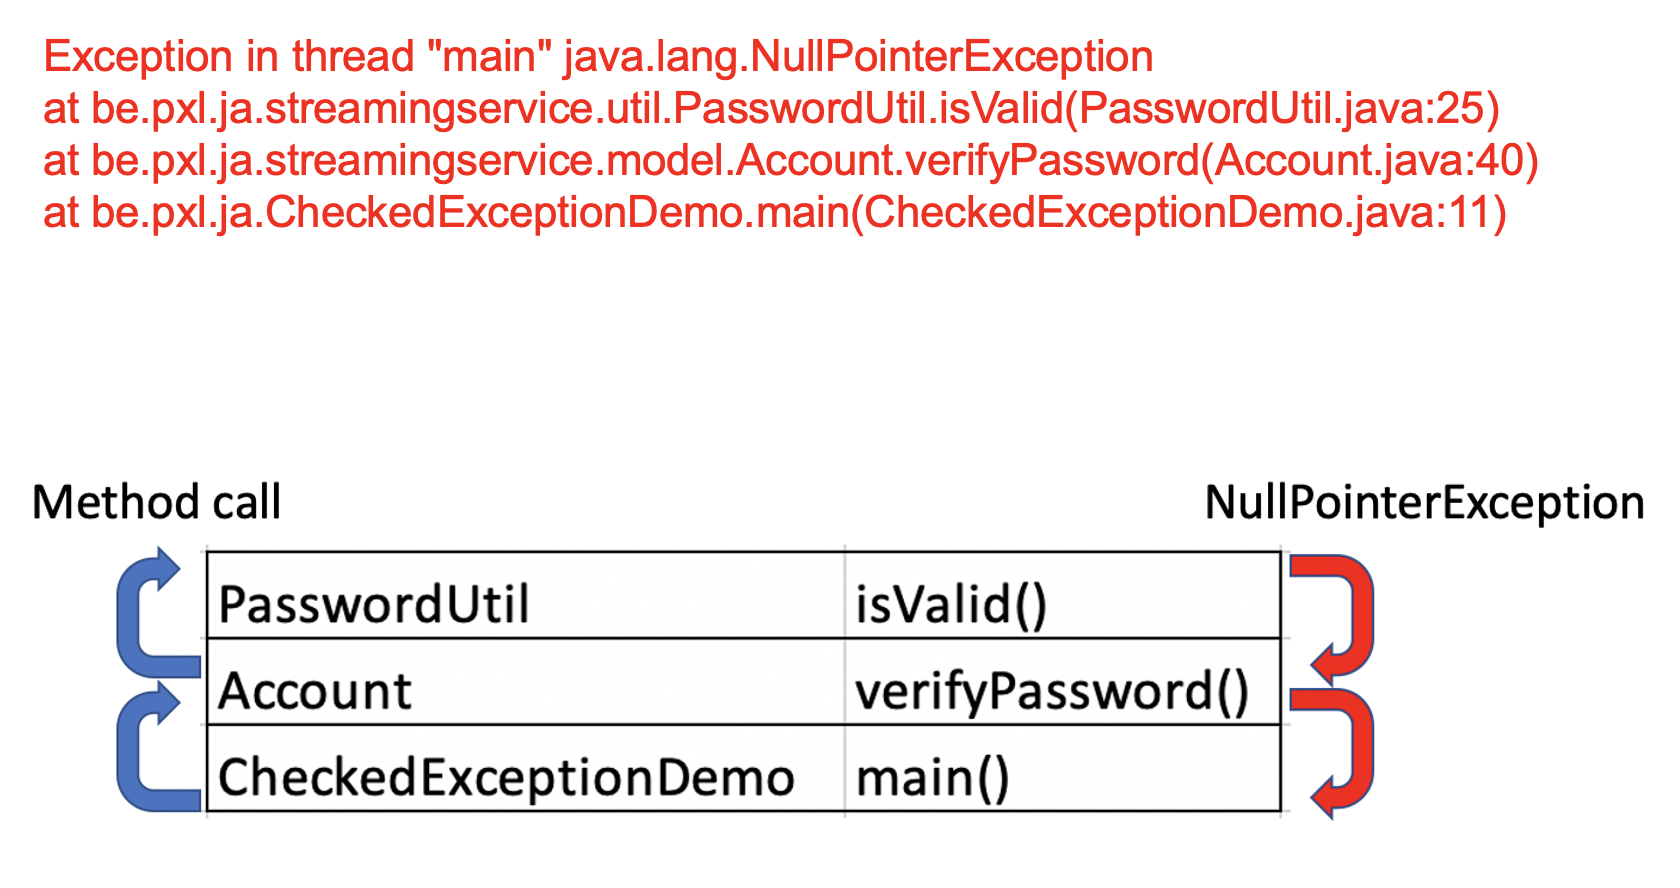
\includegraphics[width=\linewidth]{images/h2/exception_call_stack.png}
\caption{Method call stack}
\label{fig:method_call_stack}
\end{figure}

De NoSuchAlgorithmException wordt afgehandeld door null te geven als returnwaarde van de methode encodePassword.  Hierdoor wordt het probleem pas opgemerkt op het ogenblik dat we de methode isValid van de klasse PasswordUtil gebruiken. De informatie dat het foute algoritme werd meegegeven is momenteel volledig verloren gegaan. Daarom wordt altijd aangeraden om exceptions die zich voordoen in je programma bij te houden in logbestanden. Het gebruik van logbestanden valt buiten de scope van deze cursus. Als alternatief voor het loggen van exceptions zullen we in deze cursus de stacktrace van de exception tonen in de console.

\begin{lstlisting}
import java.math.BigInteger;
import java.security.MessageDigest;
import java.security.NoSuchAlgorithmException;

public class PasswordUtil {

	private static final String ALGORITHM = "MD4";

	public static String encodePassword(String password) {
		MessageDigest messageDigest = null;
		try {
			messageDigest = MessageDigest.getInstance(ALGORITHM);
		} catch (NoSuchAlgorithmException e) {
			e.printStackTrace();
			return null;
		}
		messageDigest.update(password.getBytes(), 0, password.length());
		return new BigInteger(1, messageDigest.digest()).toString(16);
	}

	public static boolean isValid(String providedPassword, String securedPassword) {
		return encodePassword(providedPassword).equals(securedPassword);
	}
}
\end{lstlisting}
 
Door de stacktrace te tonen in de console raken we geen cruciale informatie kwijt.

\begin{verbatim}
java.security.NoSuchAlgorithmException: MD4 MessageDigest not available
	at java.base/sun.security.jca.GetInstance.getInstance(GetInstance.java:159)
	at java.base/java.security.Security.getImpl(Security.java:700)
	at java.base/java.security.MessageDigest.getInstance(MessageDigest.java:177)
	at be.pxl.ja.streamingservice.util.PasswordUtil.encodePassword(PasswordUtil.java:15)
	at be.pxl.ja.streamingservice.model.Account.setPassword(Account.java:45)
	at be.pxl.ja.streamingservice.model.Account.<init>(Account.java:16)
	at be.pxl.ja.streamingservice.CheckedExceptionDemo.main(CheckedExceptionDemo.java:8)
java.security.NoSuchAlgorithmException: md4 MessageDigest not available
	at java.base/sun.security.jca.GetInstance.getInstance(GetInstance.java:159)
	at java.base/java.security.Security.getImpl(Security.java:700)
	at java.base/java.security.MessageDigest.getInstance(MessageDigest.java:177)
	at be.pxl.ja.streamingservice.util.PasswordUtil.encodePassword(PasswordUtil.java:15)
	at be.pxl.ja.streamingservice.util.PasswordUtil.isValid(PasswordUtil.java:25)
	at be.pxl.ja.streamingservice.model.Account.verifyPassword(Account.java:37)
	at be.pxl.ja.streamingservice.CheckedExceptionDemo.main(CheckedExceptionDemo.java:9)
Exception in thread "main" java.lang.NullPointerException
	at be.pxl.ja.streamingservice.util.PasswordUtil.isValid(PasswordUtil.java:25)
	at be.pxl.ja.streamingservice.model.Account.verifyPassword(Account.java:37)
	at be.pxl.ja.streamingservice.CheckedExceptionDemo.main(CheckedExceptionDemo.java:9)
\end{verbatim}

Opnieuw zie je het belang van unit testen. Een foute waarde voor het gekozen algoritme ga je al heel snel opmerken en herstellen als je unit testen schrijft voor de methoden encodePassword() en isValid().

In dit voorbeeld is het eigenlijk aangewezen om de exception niet af te handelen. Een alternatief is dat we de methode encodePassword() toelaten om de exception, als die zich voordoet, gewoon verder door te geven (gooien).
Hierdoor komt de exception dus terecht op de plaatsen waar je de methode encodePassword() gaat aanroepen en moet je op die plaatsen afhandeling voorzien. Je kan er dus voor kiezen om de checked exception NoSuchAlgorithmException helemaal mee te sleuren doorheen je applicatie tot aan de main()-methode.

\begin{lstlisting}
import java.math.BigInteger;
import java.security.MessageDigest;
import java.security.NoSuchAlgorithmException;

public class PasswordUtil {

	private static final String ALGORITHM = "MD5";

	public static String encodePassword(String password) throws NoSuchAlgorithmException {
		MessageDigest messageDigest = MessageDigest.getInstance(ALGORITHM);
		messageDigest.update(password.getBytes(), 0, password.length());
		return new BigInteger(1, messageDigest.digest()).toString(16);
	}

	public static boolean isValid(String providedPassword, String securedPassword) throws NoSuchAlgorithmException {
		return encodePassword(providedPassword).equals(securedPassword);
	}
}
\end{lstlisting}

\begin{lstlisting}
import java.security.NoSuchAlgorithmException;
import java.util.ArrayList;
import java.util.List;

public class Account {
	private String email;
	private String password;

	public Account(String email, String password) throws NoSuchAlgorithmException {
		this.email = email;
		setPassword(password);
	}

	public String getEmail() {
		return email;
	}

	public void setEmail(String email) {
		this.email = email;
	}

	public boolean verifyPassword(String password) throws NoSuchAlgorithmException {
		return PasswordUtil.isValid(password, this.password);
	}

	public void setPassword(String password) throws NoSuchAlgorithmException {
		this.password = PasswordUtil.encodePassword(password);
	}
}
\end{lstlisting}

\begin{lstlisting}
import be.pxl.ja.streamingservice.model.Account;
import java.security.NoSuchAlgorithmException;

public class CheckedExceptionDemo {

	public static void main(String[] args) throws NoSuchAlgorithmException {
		Account newAccount = new Account("daffy@duckstad.be", "daffy123!");
		System.out.println(newAccount.verifyPassword("daffy123"));
		System.out.println(newAccount.verifyPassword("daffy123!"));
	}
}
\end{lstlisting}

Je ziet dat nu bij de signatuur van verschillende methoden ``throws NoSuchAlgorithmException'' verschijnt.
Regelmatig verschijnen er artikels met titels als ``Checked exceptions: Java’s biggest mistake'' en ``Checked Exceptions are Evil'' om het gebruik van checked exceptions te ontmoedigen. 

Een laatste en nette oplossing is om de NoSuchAlgorithmException the \textbf{wrappen}  in een runtime exception bijv. een IllegalArgumentException.

\begin{lstlisting}
import java.math.BigInteger;
import java.security.MessageDigest;
import java.security.NoSuchAlgorithmException;

public class PasswordUtil {

	private static final String ALGORITHM = "MD4";

	public static String encodePassword(String password) {
		MessageDigest messageDigest = null;
		try {
			messageDigest = MessageDigest.getInstance(ALGORITHM);
		} catch (NoSuchAlgorithmException e) {
			throw new IllegalArgumentException(e);
		}
		messageDigest.update(password.getBytes(), 0, password.length());
		return new BigInteger(1, messageDigest.digest()).toString(16);
	}

	public static boolean isValid(String providedPassword, String securedPassword) {
		return encodePassword(providedPassword).equals(securedPassword);
	}
}
\end{lstlisting}

Bij het uitvoeren van de methode encodePassword() met een foutief algoritme krijg je dan een runtime exception.

\begin{verbatim}
Exception in thread "main" java.lang.IllegalArgumentException: java.security.NoSuchAlgorithmException: MD4 MessageDigest not available
	at be.pxl.ja.streamingservice.util.PasswordUtil.encodePassword(PasswordUtil.java:17)
	at be.pxl.ja.streamingservice.model.Account.setPassword(Account.java:48)
	at be.pxl.ja.streamingservice.model.Account.<init>(Account.java:18)
	at be.pxl.ja.CheckedExceptionDemo.main(CheckedExceptionDemo.java:10)
	at java.base/jdk.internal.reflect.NativeMethodAccessorImpl.invoke0(Native Method)
	at java.base/jdk.internal.reflect.NativeMethodAccessorImpl.invoke(NativeMethodAccessorImpl.java:62)
	at java.base/jdk.internal.reflect.DelegatingMethodAccessorImpl.invoke(DelegatingMethodAccessorImpl.java:43)
	at java.base/java.lang.reflect.Method.invoke(Method.java:564)
	at com.intellij.rt.execution.application.AppMainV2.main(AppMainV2.java:131)
Caused by: java.security.NoSuchAlgorithmException: MD4 MessageDigest not available
	at java.base/sun.security.jca.GetInstance.getInstance(GetInstance.java:159)
	at java.base/java.security.Security.getImpl(Security.java:700)
	at java.base/java.security.MessageDigest.getInstance(MessageDigest.java:177)
	at be.pxl.ja.streamingservice.util.PasswordUtil.encodePassword(PasswordUtil.java:15)
	... 8 more
\end{verbatim}

\section{Multi-catch blok en finally}

\begin{lstlisting}
import java.util.Scanner;

public class MultiCatchBlockDemo {

	public static void main(String[] args) {
		Scanner scanner = new Scanner(System.in);
		System.out.println("Kies een positie: ");
		int positie = scanner.nextInt();
		System.out.println("Kies een deler: ");
		int deler = scanner.nextInt();
		try {
			int getallen[] = new int[10];
			getallen[positie] = 30 / deler;
		} catch (ArrayIndexOutOfBoundsException e) {
			System.out.println("Je moet een positie kiezen tussen 0 en 9.");
		} catch (Exception e) {
			System.out.println(e.getMessage());
		} finally {
			System.out.println("Je koos positie " + positie);
		}
		System.out.println("Start je het programma nog een keer.");
	}
}
\end{lstlisting}

Een try-blok kan gevolgd worden door \'e\'en of meerder catch-blokken.
Wanneer een exception optreedt zal bij het eerste catch-blok gestart worden. Indien onze exception een instantie is van de opgevangen exception  (instanceof) dan zal dat catch-blok uitgevoerd worden en worden de volgende catch-blokken niet meer bekeken. Indien de exception geen instantie is van de opgevangen exception dan wordt er verder gekeken naar de volgende catch-blokken tot een overeenkomstig catch-blok worden gevonden. Indien er geen catch-blok wordt gevonden zal de runtime-exception doorstromen naar de aanroepende methode.

De volgorde van de catch-blokken is van belang. ArrayIndexOutOfBoundsException is een subklasse van Exception. Als we eerst een catch-blok aanmaken voor de superklasse en pas daarna een catch-blok voor de subklasse zou het tweede catch-blok ``onbereikbaar'' zijn. Het eerste catch-blok gaat de exception reeds kunnen afhandelen. Code die onbereikbaar is (unreachable code) wordt opgemerkt door de compiler wat resulteert in een compileerfout van je code.

\begin{oefening}
Wissel beide catch-blokken eens van plaats in bovenstaande code.
\end{oefening}

Het finally-blok tenslotte is een codeblok dat altijd wordt uitgevoerd: of er nu een exception optreedt of niet. Zelfs als er een exception optreedt en die niet kan worden afgehandeld door een catch-blok, zal toch het finally-blok uitgevoerd worden.

\begin{oefening}
Test de werking van het finally-blok eens uit met bovenstaand programma MultiCatchBlockDemo. Verwijder het tweede catch-blok eens en veroorzaak een deling door 0. Wat gebeurt er?
\end{oefening}

Indien je dezelfde code hebt om verschillende exceptions af te handelen, mag je exceptions combineren in een catch-block. Zo zal het catch-blok in onderstaand voorbeeld zowel ArrayIndexOutOfBoundsExceptions als ArithmeticExceptions afhandelen.

\begin{lstlisting}
public class MultipleCatches {

	public static void main(String[] args) {
		Scanner scanner = new Scanner(System.in);
		System.out.println("Kies een positie: ");
		int positie = scanner.nextInt();
		System.out.println("Kies een deler: ");
		int deler = scanner.nextInt();
		try {
			int getallen[] = new int[10];
			getallen[positie] = 30 / deler;
		} catch (ArrayIndexOutOfBoundsException | ArithmeticException e) {
			System.out.println(e.getMessage());
		}
		System.out.println("Start je het programma nog een keer.");
	}
}
\end{lstlisting}

\section{Zelf exceptions opgooien}
We willen gaan controleren dat de gebruikers van onze streaming service enkel geldige kredietkaartnummers invullen. Daarom maken we een aparte klasse CreditCardNumber. We gaan ervoor zorgen dat objecten van de klasse CreditCardNumber nooit ongeldige gegevens bevatten. Wanneer je een object van de klasse CreditCardNumber probeert aan te maken met ongeldige gegevens zal er een IllegalArgumentException gegooid worden.

We laten 2 types van kredietkaarten toe: VISA en MASTERCARD. Kaartnummers van VISA-kaarten starten altijd met het nummer 5, kaartnummers van MASTERCARD-kaarten starten altijd met 4.
Verder wordt ook gecontroleerd dat de kaartnummers bestaan uit 16 cijfers. Bestudeer de klasse CreditCardNumber.

\begin{lstlisting}
public class CreditCardNumber {
	private static final int LENGTH = 16;
	private static final int CVC_LENGTH = 3;

	private CreditCardType creditCardType;
	private String number;
	private String cvc;

	public CreditCardNumber(String number, String cvc) {
		if (!isNumeric(number) || number.length() != LENGTH) {
			throw new IllegalArgumentException("A card number must have " + LENGTH + " digits.");
		}
		creditCardType = getCreditCardType(number);
		if (creditCardType == null) {
			throw new IllegalArgumentException("This is not a valid credit card.");
		}
	}

	private boolean isNumeric(String text) {
		if (text == null || text.length() == 0) {
			return false;
		}
		try {
			Long.parseLong(text);
			return true;
		} catch (NumberFormatException e) {
			return false;
		}
	}

	private CreditCardType getCreditCardType(String number) {
		for (CreditCardType cardType : CreditCardType.values()) {
			if (cardType.getFirstNumber() == Integer.parseInt(number.substring(0, 1))) {
				return cardType;
			}
		}
		return null;
	}
}
\end{lstlisting} 

Natuurlijk gaan we de constructor van onze nieuwe klasse CreditCardNumber ook grondig testen.  Wanneer we dus foutieve waarden meegeven aan de constructor gaan we moeten verifi\"eren dat de IllegalArgumentException wordt opgegooid.

Hier is alvast een eenvoudig voorbeeld om te tonen hoe de methode assertThrows van de klasse Assertions in junit werkt.

\begin{lstlisting}
@Test
void testExpectedException() {
  Assertions.assertThrows(NumberFormatException.class, () -> {
    Integer.parseInt("One");
  });
}
\end{lstlisting}

De assertThrows() verwacht dat een NumberFormatException zal worden opgegooid. Omdat de string ``One'' een ongeldige waarde is zal de NumberFormatException ook effectief gegooid worden en zal de test dus slagen.

Nu zie je een aantal testen om onze constructor van de klasse CreditCardNumber te testen. Bestudeer de testen grondig.


\begin{lstlisting}
import org.junit.jupiter.api.Test;

import static org.junit.jupiter.api.Assertions.assertEquals;
import static org.junit.jupiter.api.Assertions.assertThrows;

public class CreditCardNumberTest {

	@Test
	public void validVisaCard() {
		CreditCardNumber creditCardNumber = new CreditCardNumber("4321876532147654", "123");

		assertEquals(CreditCardType.VISA, creditCardNumber.getType());
		assertEquals("123", creditCardNumber.getCvc());
		assertEquals("4321876532147654", creditCardNumber.getNumber());
	}

	@Test
	public void validVisaCardWithBlanks() {
		CreditCardNumber creditCardNumber = new CreditCardNumber("  43218 76532 1476 54  ", " 1 2 3 ");

		assertEquals(CreditCardType.VISA, creditCardNumber.getType());
		assertEquals("123", creditCardNumber.getCvc());
		assertEquals("4321876532147654", creditCardNumber.getNumber());
	}

	@Test
	public void validMasterCard() {
		CreditCardNumber creditCardNumber = new CreditCardNumber("5321876532147654", "123");

		assertEquals(CreditCardType.MASTERCARD, creditCardNumber.getType());
		assertEquals("123", creditCardNumber.getCvc());
		assertEquals("5321876532147654", creditCardNumber.getNumber());
	}

	@Test
	public void validMasterCardWithBlanks() {
		CreditCardNumber creditCardNumber = new CreditCardNumber("  53218 76532 1476 54  ", " 1 2 3 ");

		assertEquals(CreditCardType.MASTERCARD, creditCardNumber.getType());
		assertEquals("123", creditCardNumber.getCvc());
		assertEquals("5321876532147654", creditCardNumber.getNumber());
	}

	@Test
	public void throwsInvalidArgumentExceptionWhenNumberTooShort() {
		assertThrows(IllegalArgumentException.class, () -> {
			new CreditCardNumber("  53218 76532 1476  ", " 1 2 3 ");
		});
	}

	@Test
	public void throwsInvalidArgumentExceptionWhenNumberTooLong() {
		assertThrows(IllegalArgumentException.class, () -> {
			new CreditCardNumber("  53218 76532 1476 4445  ", " 1 2 3 ");
		});
	}

	@Test
	public void throwsInvalidArgumentExceptionWhenInvalidCardType() {
		assertThrows(IllegalArgumentException.class, () -> {
			new CreditCardNumber("7321876532147654", "123");
		});
	}
}
\end{lstlisting}

\begin{oefening}
Voeg in de constructor van de klasse CreditCardNumber een extra validatie toe voor de CVC (card validation code). De CVC is een getal bestaande uit 3 cijfers.
Pas je unit testen aan. Waarschijnlijk moet je extra unit testen toevoegen om de constructor van de klasse CreditCardNumber te testen.
\end{oefening}


\section{Zelf exception-klassen schrijven}

In de klasse CreditCardNumber hebben we gebruikgemaakt van een bestaande exception uit de JDK. We kunnen ook onze eigen Exception-klassen voorzien.

De klasse PaymentInfo gaan we nu grondig aanpassen door o.a. gebruik te maken van de klasse CreditCardNumber. Daarnaast willen we ook de vervaldatum van de kredietkaart gaan controleren. We willen namelijk dat de kredietkaart nog minstens 1 maand geldig is op het ogenblik dat de betaalgegevens worden ingegeven. Indien de vervaldatum binnen de maand valt, gaan we een InvalidDateException opgooien.

Deze InvalidDateException-klasse bestaat niet in de JDK, dus gaan we hem zelf voorzien. Wanneer je een \textbf{checked exception} wil maken gebruik je de klasse Exception als superklasse van je nieuwe exception. Wanneer je een \textbf{unchecked exception} wil maken gebruik je de klasse RuntimeException als superklasse.

Hier is alvast onze nieuwe exception klasse InvalidDateException. Als je zelf een exception klasse aanmaakt kan je zelf beslissen welke parameters en extra eigenschappen je voorziet in de constructor. Regelmatig wordt ook de afspraak gehanteerd dat er pas een nieuwe exception klasse wordt toegevoegd, indien \'e\'en van de reeds bestaande exception klassen niet eenvoudig hergebruikt kan worden. In ons geval, gaan we de ongeldige datum willen tonen. Om het samenstellen van de foutboodschap te kunnen hergebruiken is het dus zinvol om een InvalidDateException te maken met o.a. de ongeldige datum (LocalDate) als parameter.

\begin{lstlisting}
public class InvalidDateException extends RuntimeException {

	public static final DateTimeFormatter FORMATTER = DateTimeFormatter.ofPattern("dd/MM/yyyy");

	public InvalidDateException(LocalDate incorrectDate, String type, String description) {
		super(FORMATTER.format(incorrectDate) + " is not a valid " + type + ". " + description);
	}
}
\end{lstlisting}

\begin{lstlisting}
import java.time.LocalDate;

public class PaymentInfo {

	private String firstName;
	private String lastName;
	private CreditCardNumber cardNumer;
	private LocalDate expirationDate;

	public String getFirstName() {
		return firstName;
	}

	public void setFirstName(String firstName) {
		this.firstName = firstName;
	}

	public String getLastName() {
		return lastName;
	}

	public void setLastName(String lastName) {
		this.lastName = lastName;
	}

	public void setCardNumer(CreditCardNumber cardNumer) {
		this.cardNumer = cardNumer;
	}

	public LocalDate getExpirationDate() {
		return expirationDate;
	}

	public void setExpirationDate(LocalDate expirationDate) {
		if (LocalDate.now().plusMonths(1).isAfter(expirationDate)) {
			throw new InvalidDateException(expirationDate, "expirationDate", "Must be valid for at least 1 month.");
		}
		this.expirationDate = expirationDate;
	}
}
\end{lstlisting}

We gaan deze  methode setExpirationDate nu ook grondig testen.

\begin{lstlisting}
import org.junit.jupiter.api.BeforeEach;
import org.junit.jupiter.api.Test;

import java.time.LocalDate;

import static org.junit.jupiter.api.Assertions.assertEquals;
import static org.junit.jupiter.api.Assertions.assertNotNull;
import static org.junit.jupiter.api.Assertions.assertThrows;

public class PaymentInfoSetExpirationDateTest {

	private PaymentInfo paymentInfo;

	@BeforeEach
	public void init() {
		paymentInfo = new PaymentInfo();
	}

	@Test
	public void throwsInvalidDateExceptionWhenExpirationDayWithinOneMonth() {
		LocalDate withinOneMonth = LocalDate.now().plusMonths(1).minusDays(1);
		assertThrows(InvalidDateException.class, () -> paymentInfo.setExpirationDate(withinOneMonth));
	}

	@Test
	public void expirationDayWithinExactlyOneMonthIsAllowed() {
		LocalDate exactlyOneMonth = LocalDate.now().plusMonths(1);
		paymentInfo.setExpirationDate(exactlyOneMonth);

		assertNotNull(paymentInfo.getExpirationDate());
		assertEquals(exactlyOneMonth, paymentInfo.getExpirationDate());
	}

	@Test
	public void expirationDayOverOneMonthIsAllowed() {
		LocalDate overOneMonth = LocalDate.now().plusMonths(1).plusDays(1);
		paymentInfo.setExpirationDate(overOneMonth);

		assertNotNull(paymentInfo.getExpirationDate());
		assertEquals(overOneMonth, paymentInfo.getExpirationDate());
	}

}
\end{lstlisting} 

\begin{oefening}
Schrijf ook een kort programma waarin je de InvalidDateException veroorzaakt. Vang de exception op en toon de foutboodschap (message)?
\end{oefening}




\chapter{Spring Validation}
    
\fcolorbox{black}[HTML]{E9F0E9}{\parbox{\textwidth}{%
\noindent \textbf{Learning goals}\\
De junior-collega
\begin{enumerate}[nolistsep]
\item kan gebruikmaken van Spring Validation
\item kan de correcte validatieregels gebruiken
\end{enumerate}}}

Wanneer Spring Boot een HTTP-verzoek ontvangt, is het belangrijk om de gegevens die met dat verzoek zijn meegestuurd te valideren.  Spring Boot heeft voorgedefinieerde validatoren waardoor het controleren van veelvoorkomende regels eenvoudig kan gebeuren.  Zo kan Spring Boot bijvoorbeeld heel eenvoudig controleren of een e-mailadres het juiste formaat heeft of een getal binnen een bepaald bereik valt,.
In Spring Boot is het uiteraard ook mogelijk om aangepaste of eigen validatieregels te programmeren.

Om Spring Validation te gebruiken voeg je een dependency toe aan het project.

\begin{lstlisting}
<dependency>
	<groupId>org.springframework.boot</groupId>
	<artifactId>spring-boot-starter-validation</artifactId>
</dependency>
\end{lstlisting}

Hier is een lijst van de meest gebruikte annotaties.

\begin{tabularx}{\textwidth}{|l|X|}
\hline
@NotNull & om aan te duiden dat een referentie niet null mag zijn. \\
@NotEmpty & om aan te duiden dat een list elementen moet bevatten. \\
@NotBlank & om aan te duiden dat een string niet leeg mag zijn. \\
@Min and @Max & om aan te duiden dat een numerieke waarde enkel geldig is als de waarde groter of kleiner is dan een gegeven waarde.\\
@Size &  om de lengte van een string te valideren. \\
@Email & om te controleren of een string een geldig e-mailadres bevat.\\
\hline
\end{tabularx}

\begin{lstlisting}[language=java, frame=single]
package be.pxl.demo.domain;

import com.fasterxml.jackson.annotation.JsonProperty;
import jakarta.validation.constraints.Min;
import jakarta.validation.constraints.NotBlank;
import jakarta.validation.constraints.NotNull;

public class Song {
	@NotBlank
	private String title;
	@NotBlank
	private String artist;
	@JsonProperty("duration_seconds")
	@Min(value = 1, message = "Must be greater than zero")
	private int durationSeconds;
	@NotNull
	private Genre genre;
	
	...
}
\end{lstlisting}

Wanneer Spring Boot een argument vindt dat is geannoteerd met @Valid,  wordt het automatisch gevalideerd.

\begin{lstlisting}
@RestController
@RequestMapping("/playlist/songs")
public class MusicPlaylistController {

	private static final Logger LOGGER = LoggerFactory.getLogger(MusicPlaylistController.class);
	private final MusicPlaylistService musicPlaylistService;

	@Autowired
	public MusicPlaylistController(MusicPlaylistService musicPlaylistService) {
		this.musicPlaylistService = musicPlaylistService;
	}

	@PostMapping
	public void addSong(@RequestBody @Valid Song song) {
		if (LOGGER.isInfoEnabled()) {
			LOGGER.info("Adding song [" + song.getTitle() + "]");
		}
		musicPlaylistService.addSong(song);
	}
   ...
}
\end{lstlisting}

Wanneer het argument niet voldoet aan de regels dan gooit Spring Boot een exception van de klasse MethodArgumentNotValidException.

Sinds Spring Boot versie 2.3 moet je de eigenschap server.error.include-message de waarde always geven om de foutboodschappen te kunnen zien in het response. Spring Boot verbergt namelijk het foutmelding in de respons om het lekken van gevoelige informatie te voorkomen. 

De foutmelding blijft ondanks in de instelling eerder cryptisch.  Stel dat ik de REST API gebruik om een lied toe te voegen met de volgende gegevens:

\begin{verbatim}
{
  "title": "",
  "artist": "Bruno Mars",
  "duration_seconds": -2,
  "genre": "OTHER"
}
\end{verbatim}

Dan krijg je het volgende respons.

\begin{verbatim}
{
	"timestamp": "2023-09-23T13:48:50.490+00:00",
	"status": 400,
	"error": "Bad Request",
	"message": "Validation failed for object='song'. Error count: 2",
	"path": "/playlist/songs"
}
\end{verbatim}

Meer gegevens krijg ik te zien als ik de eigenschap server.error.include-binding-errors=always toevoeg in application.properties. Voor bovenstaande RequestBody krijg je dan de volgende respons. Er wordt op dat ogenblik al veel interne informatie gelekt.

\begin{lstlisting}[language=json]
{
	"timestamp": "2023-09-23T13:52:38.028+00:00",
	"status": 400,
	"error": "Bad Request",
	"message": "Validation failed for object='song'. Error count: 2",
	"errors": [
		{
			"codes": [
				"Min.song.durationSeconds",
				"Min.durationSeconds",
				"Min.int",
				"Min"
			],
			"arguments": [
				{
					"codes": [
						"song.durationSeconds",
						"durationSeconds"
					],
					"arguments": null,
					"defaultMessage": "durationSeconds",
					"code": "durationSeconds"
				},
				10
			],
			"defaultMessage": "Invalid duration_seconds: must equal or exceed 10.",
			"objectName": "song",
			"field": "durationSeconds",
			"rejectedValue": -2,
			"bindingFailure": false,
			"code": "Min"
		},
		{
			"codes": [
				"NotBlank.song.title",
				"NotBlank.title",
				"NotBlank.java.lang.String",
				"NotBlank"
			],
			"arguments": [
				{
					"codes": [
						"song.title",
						"title"
					],
					"arguments": null,
					"defaultMessage": "title",
					"code": "title"
				}
			],
			"defaultMessage": "must not be blank",
			"objectName": "song",
			"field": "title",
			"rejectedValue": "",
			"bindingFailure": false,
			"code": "NotBlank"
		}
	],
	"path": "/playlist/songs"
}
\end{lstlisting}

De best practice om de MethodArgumentNotValidException af te handelen is door gebruik te maken van een exception handler.  Hierbij gebruiken we de annotaties @RestControllerAdvice en @ExceptionHandler. 

\begin{lstlisting}
package be.pxl.demo.config;

import org.springframework.http.HttpStatus;
import org.springframework.http.ResponseEntity;
import org.springframework.validation.ObjectError;
import org.springframework.web.bind.MethodArgumentNotValidException;
import org.springframework.web.bind.annotation.ExceptionHandler;
import org.springframework.web.bind.annotation.RestControllerAdvice;

import java.util.ArrayList;
import java.util.List;

@RestControllerAdvice
public class GlobalExceptionHandler {

	@ExceptionHandler(MethodArgumentNotValidException.class)
	public ResponseEntity<List<String>> handleValidationErrors(MethodArgumentNotValidException ex) {
		List<String> errors = new ArrayList<>();
		for (ObjectError error: ex.getBindingResult().getAllErrors()) {
			errors.add(error.getDefaultMessage());
		}
		return new ResponseEntity<>(errors, HttpStatus.BAD_REQUEST);
	}
}
\end{lstlisting}


De annotatie @RestControllerAdvice geeft aan dat deze klasse verantwoordelijk is voor het afhandelen van exceptions. Alle exception worden onderschept en indien er voor het type exception een handler is gedefinieerd, zal de bijhorende code worden uitgevoerd. 

In deze klasse is er enkel een methode voorzien voor het afhandelen van MethodArgumentNotValidExceptions. De methode herkennen we aan de annotatie @ExceptionHandler. Binnen de methode wordt een lijst met de foutmeldingen (errors) gegenereerd.

We passen de foutboodschap bij iedere validatie ook best aan.  Gebruik een duidelijke foutboodschap om de gebruiker duidelijk te maken welke gegevens hij moet doorgeven.
Als je een meertalige applicatie hebt, kan je best een key (zoals title.not.blank) doorgeven aan de frontend zodat de eigenlijk foutboodschap in de juiste taal getoond kan worden.


\begin{lstlisting}
	@NotBlank(message = "title.not.blank")
	private String title;
	@Min(value = 10, message = "Invalid duration_seconds: must be equal to or exceed 10.")
	private int durationSeconds;
\end{lstlisting}

Er wordt in het geval van een MethodArgumentNotValidException een HTTP status 400 met de volgende response body gegeven:
\begin{verbatim}
[
	"Invalid duration_seconds: must be equal to or exceed 10.",
	"title.not.blank",
	"Please provide artist name."
]
\end{verbatim}


\begin{oefening}
\textbf{Huizenjacht}

We voeren een aantal aanpassingen uit aan de klasse House.
\begin{itemize}
\item Voeg de volgende eigenschappen toe:
\begin{itemize}
\item area: oppervlakte van de woning in m\textsuperscript{2}
\item epcScore: waarde uit de opsomming EPCScore.
\end{itemize}
\item Verwijder de eigenschap price. De prijs is nu een berekende waarde. Vermenigvuldig de oppervlakte met de basisprijs per m\textsuperscript{2} en het percentage behorende bij de epc score.
De huidige basisprijs per m\textsuperscript{2} is 2356.75.  Voor huizen in Hasselt en Genk is er een meerprijs van 25\%. 
\item Voeg de methode markAsSold() toe.  Deze methode verandert de status van het huis van FOR\_SALE naar SOLD. Wanneer het huis al verkocht is gooi je een IllegalStateException op.
\item Pas vervolgens de POST en PUT requests aan. Bij het toevoegen van een huis zijn de volgende velden verplicht: code, name, area (minstens 50m\textsuperscript{2}), epc-score en city. 
Bij het updaten kan je enkel volgende velden aanpassen: name, area (minstens 50m\textsuperscript{2}), city en epc-score.
\item Voorzie een aangepast endpoint /houses/\{code\}/sold om een huis als verkocht te registreren.
\end{itemize}

Test alle endpoints grondig uit.

\begin{lstlisting}[language=java]
public enum EPCScore {
	A_PLUS(1.5),
	A(1.2),
	B(1),
	C(0.98),
	D(0.90),
	E(0.80),
	F(0.75);

	private double percentage;

	EPCScore(double percentage) {
		this.percentage = percentage;
	}

	public double getPercentage() {
		return percentage;
	}
}
\end{lstlisting}

\end{oefening}


 

\printbibliography



\end{document}
